\documentclass[a4paper,oneside,12pt,final]{extreport}

% Encodage, langue
\usepackage[utf8]{inputenc}
\usepackage[french]{babel}

% Mathématiques
\usepackage{amsthm}
\usepackage{amssymb}
\usepackage{hyperref}
\hypersetup{
  colorlinks=true,
  linkcolor=black,
  urlcolor=black,
  citecolor=black,
  pageanchor=false
}

% Graphiques et figures
\usepackage{graphicx}
\usepackage{graphics}
\usepackage{adjustbox}
\usepackage{caption}
\usepackage{floatrow}
\floatsetup[table]{capposition=top}
\captionsetup[table]{position=top,skip=6pt}
\usepackage{adjustbox}
\usepackage{tikz}
\usetikzlibrary{calc}   
\usepackage{xcolor}
\definecolor{emsigreen}{HTML}{009B4D}

% Couleurs et tableaux
\usepackage[table]{xcolor}
\usepackage{colortbl}
\usepackage{array}
\usepackage{booktabs}
\usepackage{tabularx}
\definecolor{titlegray}{HTML}{595959}  % gris du titre du rapport
\definecolor{rulegray}{HTML}{3F3F3F}   % gris des filets encadrant le titre
% Couleurs page de garde officielle EMSI
\definecolor{emsicover}{HTML}{00B050}    % vert triangles + filet
\definecolor{coverbox}{HTML}{D6EFE1}     % boites vert clair
\definecolor{covergray}{HTML}{404040}    % gris du grand titre
\definecolor{coverborder}{HTML}{BFBFBF}  % bordures du tableau
% (optionnel) vert un peu plus vif, plus proche du modèle :
% \definecolor{emsigreen}{HTML}{00A651}

% Listes
\usepackage{enumitem}
\setlist[itemize]{nosep, leftmargin=*, topsep=2pt, partopsep=0pt}
\setlist[enumerate]{nosep, leftmargin=*, topsep=2pt, partopsep=0pt}

% Algorithmes
\usepackage[
  lined,
  boxed,
  commentsnumbered,
  french,
  ruled,
  vlined,
  linesnumbered
]{algorithm2e}

% Arbres et diagrammes
\usepackage{tikz}
\usepackage{tikz-qtree}
\usepackage[edges]{forest}
\usepackage{dirtree}
\usepackage{pgfgantt}

% Glossaire et index
\usepackage{makeidx}
\usepackage[acronym,toc,section=chapter]{glossaries}
\usepackage[nottoc]{tocbibind}

% Outils divers
\usepackage{etoolbox}
\usepackage{ifxetex}
\usepackage{fancyhdr}
\usepackage{pdfpages}

\parindent 0cm
\makeindex
\makeglossaries

% Page layout
\textwidth 18cm
\textheight 24cm
\topmargin -0.5cm
\oddsidemargin -1cm
\setlength{\headheight}{14.5pt}

% Font encoding
\ifxetex
  \usepackage{fontspec}
\else
  \usepackage[T1]{fontenc}
  \usepackage{lmodern}
\fi

% Theorem environments
\newtheorem{theorem}{Theorem}[chapter]
\newtheorem{definition}{Definition}[chapter]
\newtheorem{exemple}{Example}[chapter]

% Keywords commands
\providecommand{\keywords}[1]{\textbf{\textit{Mots clés---}} #1}
\providecommand{\keywordss}[1]{\textbf{\textit{Keywords---}} #1}

%% Style des têtes de chapitre
\makeatletter
% Chapitres NUMÉROTÉS : page-titre pleine page, centrée verticalement
\def\@makechapterhead#1{%
  \thispagestyle{plain}%
  \vspace*{\fill}
  {\parindent\z@\raggedright\normalfont
    {\sffamily\bfseries\fontsize{15}{18}\selectfont
       \textcolor{emsigreen}{CHAPITRE\ \thechapter}}\par
    \vskip 6pt
    {\color{emsigreen}\rule{\textwidth}{2pt}}\par
    \vskip 24pt
    {\bfseries\fontsize{30}{36}\selectfont
       \textcolor{black}{#1}\par}
    \vskip 18pt
    {\color{emsigreen!60}\rule{0.45\textwidth}{1.2pt}}\par
  }
  \vspace*{\fill}\vspace*{\fill}
}
% Chapitres NON numérotés (Introduction, Conclusion, Remerciements, ToC...) :
% en-tête en haut de page, le texte suit immédiatement
\def\@makeschapterhead#1{%
  {\parindent\z@\raggedright\normalfont
    \vspace*{12pt}
    {\bfseries\fontsize{24}{28}\selectfont
       \textcolor{black}{#1}\par}
    \vskip 8pt
    {\color{emsigreen}\rule{0.45\textwidth}{2pt}}\par
    \vskip 22pt
  }
}
\makeatother

% Headers for body chapters
\renewcommand{\chaptermark}[1]{\markboth{#1}{}}
\fancypagestyle{bodychapters}{%
  \fancyhf{}%
  \fancyhead[L]{\nouppercase{%
    \ifnum\value{chapter}>0
      \textcolor{emsigreen}{\small\bfseries Chapitre~\thechapter\ \textbf{--}\ \leftmark}%
    \fi}}%
  \fancyfoot[C]{\thepage}%
  \renewcommand{\headrulewidth}{0.4pt}%
  \renewcommand{\footrulewidth}{0pt}%
}

% ========================================
% INFORMATIONS DU DOCUMENT
% ========================================
\newcommand{\reportTitle}{\textsc{Projet de Fin d'\'etudes}}

\newcommand{\reportAuthor}{Haitham \textsc{El Abdioui}}

\newcommand{\reportSubject}{Contribution \`a la conception et au d\'eveloppement de la plateforme de gestion des devis BIFR\"OST}
\newcommand{\academicYearLong}{2025 / 2026}

\newcommand{\dateSoutenance}{16/07/2026}

\newcommand{\academicYear}{2025--2026}

\newcommand{\studyDepartment}{VISEO}

\newcommand{\EMSI}{\'Ecole Marocaine des Sciences de l'Ing\'enieur}

% Encadrants
\newcommand{\juryMemberOne}{M. Nabil \textsc{El Ouardi}}
\newcommand{\juryMemberOneDesc}{Encadrant Acad\'emique}

\newcommand{\juryMemberTwo}{Mme Jihad \textsc{Doumiri}}
\newcommand{\juryMemberTwoDesc}{Consultante .NET}

% Membres du jury
\newcommand{\juryMemberThree}{FLAN \textsc{FLANE}}
\newcommand{\juryMemberThreeDesc}{POSTE}

\newcommand{\juryMemberFour}{FLANE \textsc{FLANE}}
\newcommand{\juryMemberFourDesc}{FLANE}

\newcommand{\juryMemberFive}{FLANE \textsc{FLANE}}
\newcommand{\juryMemberFiveDesc}{FLANE}

% Utility commands
\newcommand{\specialcell}[1]{%
  \begin{tabularx}{\textwidth}{@{}X@{}}#1\end{tabularx}%
}

% Document metadata
\title{\reportSubject}
\author{\reportAuthor}

% Acronyms
\newacronym{api}{API}{Application Programming Interface}
\newacronym{efc}{EFC}{Entity Framework Core}
\newacronym{ci}{CI}{Continuous Integration}

\pagenumbering{roman}
\setcounter{page}{0}

\begin{document}

% ===== Page de garde importée depuis le PDF officiel =====
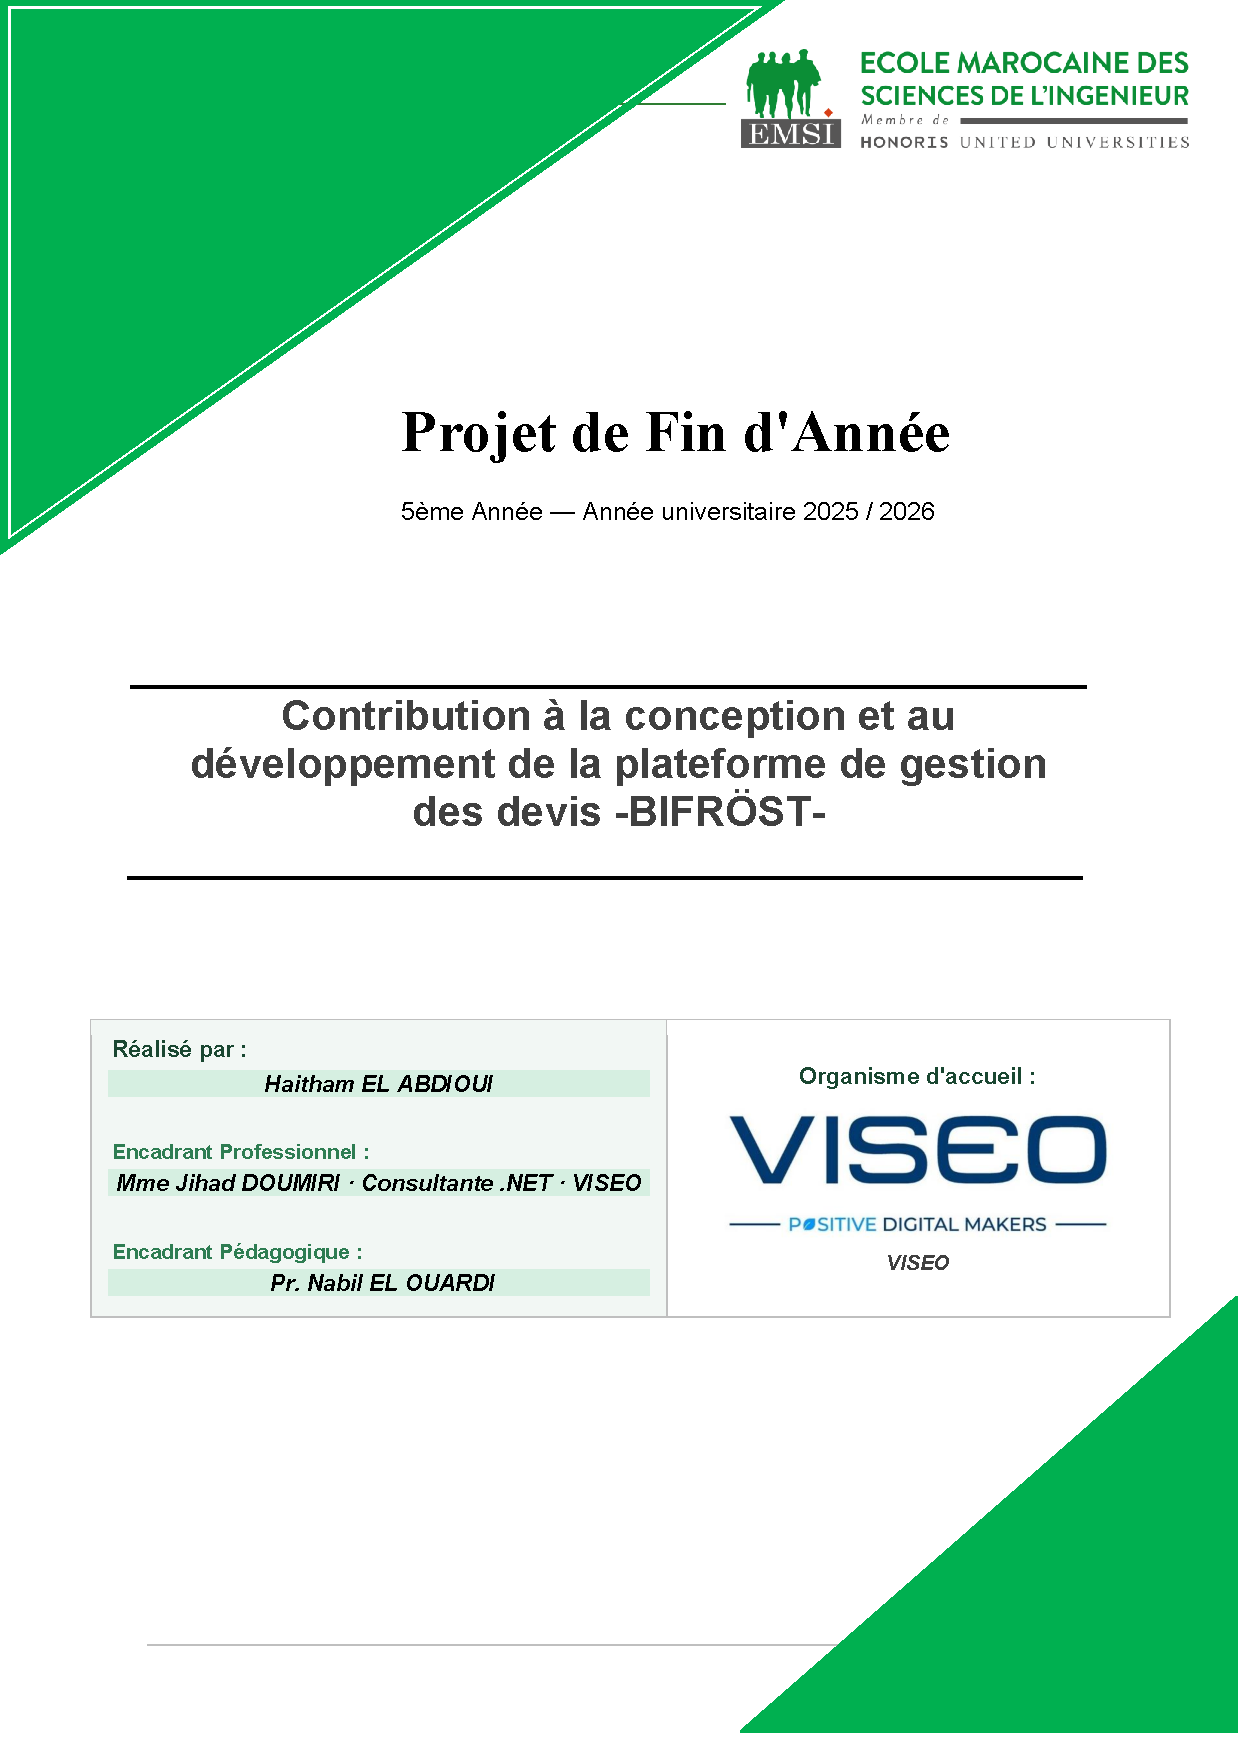
\includepdf[pages=1,fitpaper=true]{image/Page_de_garde.pdf}
\hypersetup{pageanchor=true}

% ========================================
% DÉDICACE
% ========================================
\chapter*{D\'edicace}
\thispagestyle{empty}

\vspace*{1.5cm}
\begin{center}
\itshape

À mes très chers parents,\\[0.4cm]
Aucun mot ne saurait exprimer ma profonde gratitude pour votre amour inconditionnel.\\
Vos prières, vos sacrifices et votre soutien indéfectible ont été ma lumière et ma force.\\
Que ce modeste travail soit le fruit de vos efforts et une source de fierté pour vous.\\[1cm]

À mes s\oe{}urs et à toute ma famille,\\[0.4cm]
Pour votre présence réconfortante, vos encouragements constants et la joie que vous m'apportez.\\
Dans les moments de doute comme dans les moments de joie, vous avez toujours été là.\\[1cm]

À mes chers amis et camarades ,\\[0.4cm]
Pour les précieux moments de partage, l'entraide et les souvenirs inoubliables qui ont marqué\\
ces années d'études.\\[1cm]

À toutes les personnes qui ont contribué, de près ou de loin, à mon accomplissement\\
personnel et professionnel.\\[1.5cm]

\textbf{\Large Merci.}

\end{center}

% ========================================
% REMERCIEMENTS
% ========================================
\chapter*{Remerciements}
\thispagestyle{empty}


Au terme de ce travail, je tiens à exprimer ma profonde gratitude à toutes les personnes qui ont contribué, de près ou de loin, à la réalisation de ce projet de fin d'études.
\vspace{0.5cm}
Je souhaite remercier en premier lieu \textbf{Mme Asmaa ROUDANE}, mon encadrante académique à l'EMSI, pour ses conseils judicieux, sa disponibilité constante et son accompagnement tout au long de ce projet. Ses orientations m'ont permis de mener à bien cette étude dans les meilleures conditions.
\vspace{0.5cm}
Mes sincères remerciements vont également à \textbf{Mr Abdellah LAMBARAA}, mon encadrant entreprise chez OCP Maintenance Solutions, pour m'avoir accueilli au sein de son équipe et pour la confiance qu'il m'a accordée. Son expertise technique et sa connaissance approfondie des processus de sûreté industrielle ont été déterminantes pour l'aboutissement de ce travail.
\vspace{0.5cm}
Je remercie chaleureusement toute l'équipe d'\textbf{OCP Maintenance Solutions} pour leur accueil bienveillant, leur collaboration et pour avoir mis à ma disposition tous les moyens nécessaires à la réalisation de ce projet. Leur professionnalisme et leur esprit d'équipe ont rendu cette expérience particulièrement enrichissante.
\vspace{0.5cm}
Ma reconnaissance s'adresse également à tous les enseignants de l'\textbf{École Marocaine des Sciences de l'Ingénieur (EMSI)} qui m'ont transmis leurs connaissances et m'ont préparé à relever les défis du monde professionnel.
\vspace{0.5cm}
Enfin, je ne saurais oublier de remercier ma famille et mes proches pour leur soutien inconditionnel, leurs encouragements et leur patience tout au long de mon parcours académique.


% ========================================
% RÉSUMÉ
% ========================================
\chapter*{Résumé}
\thispagestyle{empty}

Dans un contexte industriel où la sécurité et la digitalisation constituent des enjeux majeurs, l'Office Chérifien des Phosphates (OCP) s'engage dans une démarche d'amélioration continue de ses processus de gestion des accès et de sûreté industrielle. Ce projet de stage s'inscrit dans cette dynamique en contribuant au développement et à l'optimisation du système JLHUBSECURITY chez OCP Maintenance Solutions.

\vspace{0.5cm}

Les processus traditionnels de gestion des accès au site de Jorf Lasfar présentaient plusieurs limitations : saisies manuelles répétitives sources d'erreurs, temps d'attente prolongés aux heures de pointe, absence de traçabilité numérique et risque de perte des pièces d'identité des visiteurs. Ces dysfonctionnements impactaient l'efficacité opérationnelle et la satisfaction des utilisateurs.

\vspace{0.5cm}

 L'objectif principal consistait à digitaliser et moderniser le système de gestion des accès en développant une plateforme web intégrée permettant de dématérialiser les demandes, automatiser les workflows de validation, générer des badges QR code sécurisés et améliorer l'expérience utilisateur.
 
\vspace{0.5cm}

Le projet a été mené selon une approche agile avec analyse des besoins utilisateurs, étude des processus existants, conception d'une architecture technique robuste et développement d'une solution modulaire. La stack technique retenue comprend Laravel pour le backend et Vue.js pour le frontend, garantissant performance et maintenabilité.

\vspace{0.5cm}

La solution développée intègre plusieurs modules fonctionnels : gestion des visiteurs avec génération automatique de QR codes, système de validation multi-niveaux, tableau de bord de pilotage, gestion des véhicules et du matériel, ainsi qu'un module spécialisé pour la ferraille. L'interface responsive assure une utilisation optimale sur tous les supports.

\vspace{0.5cm}

 L'implémentation du système JLHUBSECURITY a permis de réduire significativement les temps de traitement des demandes, d'éliminer les erreurs de saisie manuelle, d'améliorer la traçabilité des accès et d'offrir une meilleure expérience utilisateur. Les fonctionnalités de reporting et d'audit renforcent le contrôle et la supervision des activités.
 
\vspace{0.5cm}

Ce projet démontre l'importance de la transformation digitale dans l'industrie et contribue à positionner OCP comme un leader en matière d'innovation technologique appliquée à la sûreté industrielle.




% ========================================
% TABLES DES MATIÈRES
% ========================================
\newpage
\tableofcontents

\newpage
\listoffigures

\newpage
\listoftables

\cleardoublepage
\newpage
\pagenumbering{arabic}

% ========================================
% INTRODUCTION
% ========================================
\pagestyle{bodychapters}
\chapter*{Introduction G\'en\'erale}
\label{chap:introduction_generale}
\addcontentsline{toc}{chapter}{Introduction G\'en\'erale}

Dans un contexte \'economique marqu\'e par une acc\'el\'eration de la transformation num\'erique, les entreprises de services et d'int\'egration logicielle font face \`a des exigences croissantes en mati\`ere de fiabilit\'e, de maintenabilit\'e et d'exp\'erience utilisateur. Les outils m\'etier internes, longtemps consid\'er\'es comme des projets secondaires, sont devenus des leviers strat\'egiques d'efficacit\'e op\'erationnelle, dont la qualit\'e conditionne directement la productivit\'e des \'equipes qui les utilisent au quotidien.

C'est dans ce contexte que s'inscrit le stage r\'ealis\'e au sein de \textbf{VISEO}, soci\'et\'e fran\c{c}aise de conseil et d'int\'egration num\'erique, sur le projet \textbf{Bifr\"ost}~: une plateforme web de gestion de devis et d'abonnements d\'edi\'ee aux agents du service client. Bifr\"ost repose sur une architecture h\'et\'erog\`ene combinant un backend Python~/ Django REST Framework, une API .NET ASP.NET Core et un frontend Vue.js~/ TypeScript -- une combinaison qui offre flexibilit\'e et robustesse, mais impose une discipline d'\'equipe rigoureuse en mati\`ere de tests, de CI/CD et de qualit\'e de code.

La probl\'ematique centrale de ce projet r\'eside dans la capacit\'e \`a contribuer efficacement \`a un produit logiciel en production~: corriger des anomalies sans introduire de r\'egressions, implanter de nouvelles fonctionnalit\'es dans le respect de l'architecture existante, et am\'eliorer progressivement la qualit\'e du code sans d\'estabiliser les flux en cours d'utilisation. Cette contrainte, propre aux projets en TMA (Tierce Maintenance Applicative), a guid\'e l'ensemble des d\'ecisions techniques tout au long du stage.

Le pr\'esent rapport s'articule autour de quatre chapitres principaux. Le \textbf{premier chapitre} pr\'esente l'entreprise d'accueil VISEO, son positionnement et le contexte dans lequel s'inscrit le projet Bifr\"ost. Le \textbf{deuxi\`eme chapitre} analyse l'existant technique~: architecture, stack, organisation des \'equipes et processus de d\'eveloppement. Le \textbf{troisi\`eme chapitre} d\'etaille les r\'ealisations techniques effectu\'ees sur les trois couches de l'application (frontend, API .NET, backend Django), en explicitant les choix d'impl\'ementation et les contraintes rencontr\'ees. Enfin, le \textbf{quatri\`eme chapitre} aborde les perspectives d'\'evolution, notamment l'initiative d'observabilit\'e et la strat\'egie de mise \`a jour des d\'ependances Python.

% ========================================
% CHAPITRES PRINCIPAUX
% ========================================

\label{chap:1}
% ========================================
% CHAPITRE 1 - PRÉSENTATION DE L'ENTREPRISE D'ACCUEIL
% ========================================

\chapter{Présentation de l'Entreprise d'Accueil}
\label{chap:presentation_entreprise}

\section*{Introduction}

Ce premier chapitre présente l'organisme d'accueil de manière générale et détermine les objectifs et le contexte du stage. Nous commencerons par une présentation succincte du Groupe OCP, avant de nous concentrer sur OCP Maintenance Solutions, la filiale qui nous a accueillis pour ce projet de fin d'études.

Cette présentation permettra de comprendre l'environnement industriel et technologique dans lequel s'inscrit le projet JLHUBSECURITY, ainsi que les enjeux stratégiques qui sous-tendent le développement de solutions digitales innovantes dans le domaine de la sûreté industrielle.

\section{Présentation Générale du Groupe OCP}

\subsection{Introduction au Groupe OCP}

\begin{figure}[h]
\centering

\includegraphics[width=0.4\textwidth]{image/OCP-logo.jpg}
\caption{Logo du Groupe OCP}
\label{fig:logo_ocp}
\end{figure}

L'Office Chérifien des Phosphates (OCP), créé le 7 août 1920 par dahir royal, constitue aujourd'hui l'un des piliers de l'économie marocaine et un acteur incontournable sur la scène internationale. Transformé en société anonyme (OCP SA) en 2008, le groupe s'est imposé comme le leader mondial incontesté dans l'industrie des phosphates et des engrais phosphatés.

\subsubsection{Chiffres Clés du Groupe}

OCP détient une position dominante sur le marché mondial des phosphates avec des indicateurs impressionnants :

\begin{itemize}
\item \textbf{Réserves mondiales} : Accès à plus de 70\% des réserves mondiales de roches phosphatées
\item \textbf{Effectifs} : Près de 23 000 employés
\item \textbf{Part de marché} : 31\% du marché mondial des produits phosphatés
\item \textbf{Production} : Plus de 25 millions de tonnes de phosphate brut par an
\end{itemize}

\subsection{Historique du Groupe OCP}

\subsubsection{Étapes Clés de l'Évolution}

\textbf{1920-1950 : Fondation et premiers développements}
\begin{itemize}
\item \textbf{1920} : Création de l'Office Chérifien des Phosphates par dahir royal le 7 août
\item \textbf{1921} : Début de l'exploitation souterraine sur le gisement des Oulad Abdoun et première exportation de phosphate depuis Casablanca (7 000 tonnes)
\item \textbf{1930} : Ouverture du centre de production de Youssoufia
\end{itemize}

\textbf{1951-1975 : Expansion et modernisation}
\begin{itemize}
\item \textbf{1951} : Démarrage de l'extraction à ciel ouvert à Khouribga et développement des installations de séchage
\item \textbf{1965} : Création de Maroc Chimie et début de la valorisation des phosphates avec l'usine de Safi
\item \textbf{1975} : Formation du Groupe OCP et intégration des industries chimiques aux structures internes
\end{itemize}

\textbf{2008-Présent : Transformation moderne}
\begin{itemize}
\item \textbf{2008} : Transformation historique en société anonyme (OCP SA)
\item \textbf{2014} : Inauguration du pipeline de transport reliant Khouribga à Jorf Lasfar (187 km)
\item \textbf{2024} : Création d'OCP Nutricrops, nouvelle filiale spécialisée
\end{itemize}

\subsection{Structure Organisationnelle}

\begin{figure}[h]
\centering
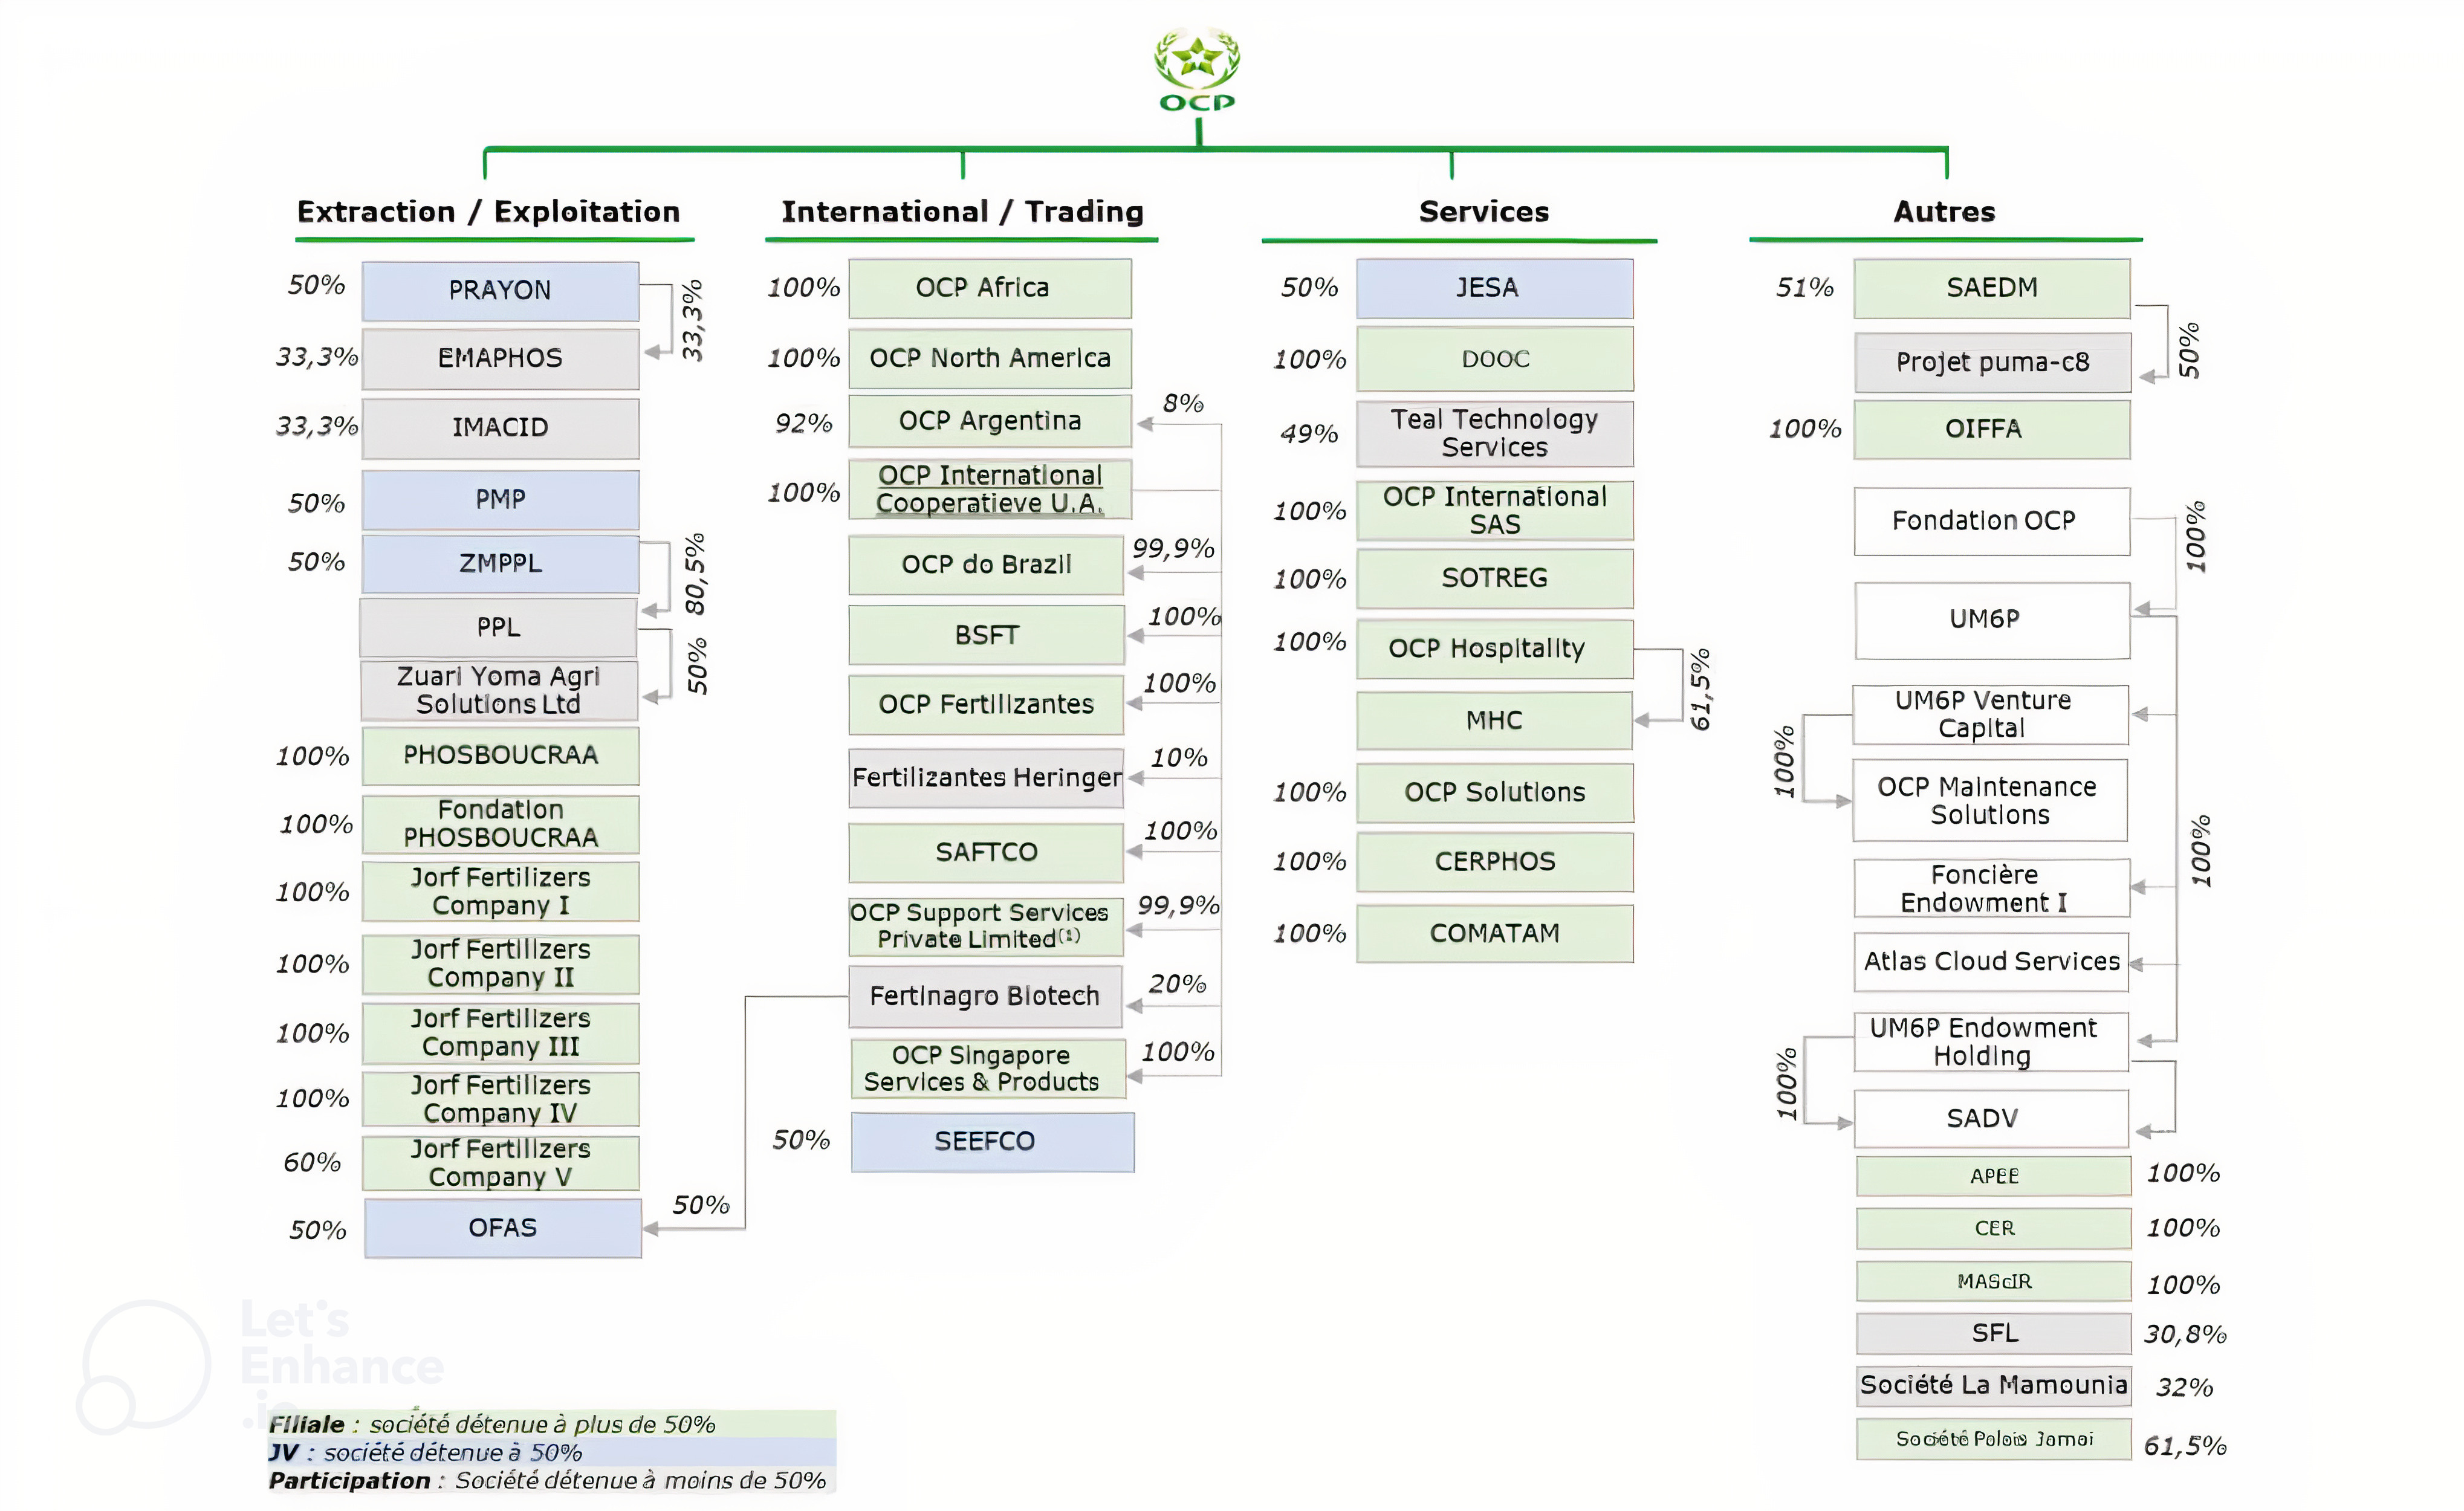
\includegraphics[width=0.8\textwidth]{image/organigramme_ocp.jpg}
\caption{Structure organisationnelle du Groupe OCP avec ses principales filiales}
\label{fig:structure_ocp}
\end{figure}
\newpage

Le Groupe OCP s'appuie sur un écosystème de filiales spécialisées, notamment \textbf{OCP Maintenance Solutions} qui constitue la filiale d'accueil de notre stage et se spécialise dans la digitalisation et la maintenance industrielle 4.0.

\section{OCP Maintenance Solutions : Notre Organisme d'Accueil}

\subsection{Présentation Générale}

\begin{figure}[h]
\centering

\includegraphics[width=0.5\textwidth]{image/ocpms.png}
\caption{Logo d'OCP Maintenance Solutions}
\label{fig:logo_ocp_ms}
\end{figure}

OCP Maintenance Solutions (OCP-MS) représente l'incarnation de la stratégie d'innovation et de digitalisation du Groupe OCP. \textbf{Créée en 2017} comme Business Unit puis transformée en filiale autonome, cette société spécialisée dans la maintenance et la digitalisation industrielle s'est rapidement imposée comme le leader marocain dans les systèmes de surveillance conditionnelle et les services de maintenance prédictive.

\subsection{Mission et Vision Stratégique}

\subsubsection{Mission d'OCP-MS}

La mission d'OCP-MS s'articule autour de trois axes stratégiques fondamentaux :

\textbf{Amélioration de la Productivité :}
\begin{itemize}
\item Optimisation des performances industrielles par l'intégration de technologies avancées
\item Réduction des temps d'arrêt non planifiés de 40\% en moyenne
\item Augmentation de la disponibilité des équipements de 15 à 20\%
\item Optimisation des coûts de maintenance de 25\% grâce à la prédictivité
\end{itemize}

\textbf{Digitalisation et Transformation :}
\begin{itemize}
\item Accompagnement complet de la transformation numérique des entreprises industrielles
\item Développement de solutions IoT et d'intelligence artificielle adaptées au contexte industriel
\item Intégration de plateformes de gestion des données industrielles
\item Mise en place de jumeaux numériques pour les équipements critiques
\end{itemize}

\textbf{Formation et Développement des Compétences :}
\begin{itemize}
\item Développement de l'expertise en maintenance industrielle 4.0
\item Certification des techniciens aux nouvelles technologies
\item Transfert de savoir-faire et de bonnes pratiques
\item Création d'un écosystème de compétences en maintenance prédictive
\end{itemize}

\subsection{Domaines d'Expertise et Solutions Technologiques}

\subsubsection{Maintenance Prédictive et Intelligence Artificielle}



OCP Maintenance Solutions a développé un écosystème technologique complet utilisant les technologies de pointe :

\textbf{Technologies Core :}
\begin{itemize}
\item \textbf{IIOT (Industrial Internet of Things)} : Capteurs intelligents connectés pour collecte de données en temps réel
\item \textbf{Big Data Analytics} : Traitement et analyse de téraoctets de données industrielles
\item \textbf{Machine Learning} : Algorithmes d'apprentissage automatique pour la détection d'anomalies
\item \textbf{Intelligence Artificielle} : Modèles prédictifs avancés pour anticiper les pannes
\end{itemize}

\textbf{Portefeuille de Solutions :}

\textbf{I-SENSE Platform :}
\begin{itemize}
\item Plateforme IoT hautement évolutive et sécurisée
\item Connexion en temps réel de milliers d'équipements
\item Interface web et mobile pour monitoring à distance
\item Tableaux de bord personnalisables par métier
\item Alertes intelligentes et notifications automatiques
\end{itemize}

\textbf{Vibox - Système de Surveillance Conditionnelle :}
\begin{itemize}
\item Protection des machines contre les dommages
\item Surveillance continue de la vibration, température, pression
\item Analyses spectrales avancées
\item Diagnostic automatique des défauts
\item ROI démontré de 300\% en moyenne
\end{itemize}

\textbf{MobiVib - Analyse Vibratoire Mobile :}
\begin{itemize}
\item Kit portable d'acquisition de données
\item Analyse spectrale sur site
\item Mesures haute précision pour équipements rotatifs
\item Rapports automatiques de diagnostic
\item Formation intégrée des opérateurs
\end{itemize}

\subsubsection{Technologies d'Inspection Avancées}

\textbf{Drones d'Inspection Industrielle :}



Acquise en août 2023, cette technologie révolutionnaire permet :

\begin{itemize}
\item \textbf{Inspection thermique} : Détection des points chauds et fuites énergétiques
\item \textbf{Inspection visuelle} : Caméras haute définition pour contrôles visuels
\item \textbf{Zones d'application} : Lignes électriques, panneaux photovoltaïques, pipelines, réservoirs
\item \textbf{Sécurité} : Élimination des risques pour le personnel en environnements dangereux
\item \textbf{Efficacité} : Réduction de 80\% du temps d'inspection
\end{itemize}

\subsubsection{Contrôles Non Destructifs (CND)}

OCP Maintenance Solutions propose une gamme complète de services CND certifiés :

\textbf{Techniques Disponibles :}
\begin{itemize}
\item \textbf{Ultrasons (UT)} : Détection de défauts internes, mesure d'épaisseurs
\item \textbf{Magnétoscopie (MT)} : Contrôle des matériaux ferromagnétiques
\item \textbf{Ressuage (PT)} : Détection de défauts de surface
\item \textbf{Radiographie industrielle (RT)} : Contrôle volumétrique des soudures
\item \textbf{Ultrasons phased array (PAUT)} : Inspection avancée des structures complexes
\item \textbf{Endoscopie industrielle} : Inspection visuelle des espaces confinés
\end{itemize}

\textbf{Secteurs d'Application :}
\begin{itemize}
\item Pétrochimie et raffinerie
\item Centrales électriques
\item Industrie minière
\item Construction métallique
\item Aéronautique
\end{itemize}

\subsection{Formation et Certification - OCP MS Academy}

\subsubsection{Centre d'Excellence en Formation}

\begin{figure}[h]
\centering

\includegraphics[width=0.4\textwidth]{image/ocp_ms_academy.png}
\caption{Centre de formation OCP MS Academy}
\label{fig:ocp_ms_academy}
\end{figure}

OCP MS Academy représente le bras formation de la filiale, avec une approche innovante basée sur le "blended learning" :

\textbf{Programmes de Formation :}
\begin{itemize}
\item \textbf{Analyse vibratoire} : Niveaux I, II, III selon standards ISO 18436
\item \textbf{Maintenance prédictive} : Techniques et technologies émergentes
\item \textbf{IoT industriel} : Déploiement et gestion de capteurs connectés
\item \textbf{Contrôles non destructifs} : Certification selon normes internationales
\item \textbf{Leadership industriel} : Management et soft skills pour l'industrie 4.0
\end{itemize}

\textbf{Méthodologie Pédagogique :}
\begin{itemize}
\item Formation présentielle avec simulateurs industriels
\item E-learning interactif et adaptatif
\item Réalité virtuelle pour situations dangereuses
\item Compagnonnage sur site avec experts
\item Certification continue et évaluation des compétences
\end{itemize}

\subsubsection{Partenariats Internationaux Stratégiques}

\textbf{Mobius Institute (Australie) :}
\begin{itemize}
\item Premier centre certificateur Mobius au Maroc et en Afrique
\item Standards internationaux en analyse vibratoire
\item Plus de 500 techniciens certifiés depuis 2020
\item Reconnaissance mondiale des certifications délivrées
\end{itemize}

\textbf{Nucleom (Canada) :}
\begin{itemize}
\item Partenariat signé en 2021 pour les CND avancés
\item Expertise en inspection de niveau NASA et aerospace
\item Transfert de technologies de pointe
\item Accès aux marchés aéronautique et nucléaire
\end{itemize}

\textbf{Autres Partenaires Technologiques :}
\begin{itemize}
\item \textbf{Wikitude (Autriche)} : Solutions de réalité augmentée
\item \textbf{ifm (Allemagne)} : Capteurs et automatismes industriels
\item \textbf{LARES (Maroc)} : Instruments de métrologie
\item \textbf{BCG Gamma (International)} : Analytics et data science
\end{itemize}

\subsection{Clientèle et Marchés}

\subsubsection{Portefeuille Clients Diversifié}



\textbf{Secteurs d'Intervention :}

\textbf{Cimenterie :}
\begin{itemize}
\item \textbf{Lafarge Holcim} : Contrat de maintenance prédictive sur 5 sites
\item \textbf{Ciments du Maroc} : Surveillance conditionnelle des broyeurs
\item Services : Analyse vibratoire, thermographie, équilibrage
\end{itemize}

\textbf{Sidérurgie et Métallurgie :}
\begin{itemize}
\item \textbf{Universal Industrial Steel} : Partenariat pluriannuel
\item \textbf{Sonasid} : Maintenance prédictive des laminoirs
\item Résultats : Réduction de 60\% des arrêts non planifiés
\end{itemize}

\textbf{Énergie et Utilities :}
\begin{itemize}
\item \textbf{ONEE} : Inspection des centrales thermiques
\item \textbf{Nareva} : Maintenance éoliennes et solaire
\item \textbf{TAQA} : Optimisation des turbines gaz
\end{itemize}

\textbf{Pétrochimie :}
\begin{itemize}
\item \textbf{SAMIR} : Expertise en raffinerie
\item \textbf{Shell Maroc} : Partenariat technologique
\item Spécialités : CND, analyse d'huile, thermographie
\end{itemize}

\textbf{International :}
\begin{itemize}
\item \textbf{Afrique de l'Ouest} : Nigeria, Sénégal, Côte d'Ivoire
\item \textbf{Maghreb} : Tunisie, Algérie (projets pilotes)
\item \textbf{Moyen-Orient} : Émirats Arabes Unis (prospection)
\end{itemize}

\subsubsection{Témoignages Clients}

\begin{quote}
\textit{"La collaboration entre Universal Industrial Steel et OCP Maintenance Solutions dure depuis plusieurs années. Les experts d'OCP-MS nous procurent des analyses pertinentes qui nous ont permis d'améliorer la disponibilité de notre outil industriel et de réaliser des économies considérables."} 

--- Directeur Technique, Universal Industrial Steel
\end{quote}

\begin{quote}
\textit{"Les experts OCP MS sont dévoués et prêts à supporter les équipes opérationnelles pour atteindre une maintenance World Class."} 

--- Responsable Maintenance, Lafarge Holcim
\end{quote}

\subsection{Innovation et Recherche \& Développement}

\subsubsection{Laboratoire d'Innovation}

OCP Maintenance Solutions dispose d'un centre R\&D dédié au développement de solutions "Made in Morocco" :

\textbf{Axes de Recherche :}
\begin{itemize}
\item \textbf{Maintenance 5.0} : Intégration de l'humain dans l'industrie 4.0
\item \textbf{Jumeaux numériques} : Modélisation virtuelle des équipements industriels
\item \textbf{IA explicable} : Algorithmes transparents pour l'aide à la décision
\item \textbf{Edge computing} : Traitement local des données pour réactivité optimale
\end{itemize}

\textbf{Projets de R\&D en Cours :}
\begin{itemize}
\item Développement d'un assistant virtuel pour techniciens de maintenance
\item Plateforme de réalité augmentée pour formation immersive
\item Algorithmes d'optimisation énergétique par IA
\item Solutions de cybersécurité pour l'IoT industriel
\end{itemize}

\subsubsection{Propriété Intellectuelle}

\begin{itemize}
\item \textbf{Brevets déposés} : 5 brevets en cours d'examen
\item \textbf{Solutions propriétaires} : 12 logiciels développés en interne
\item \textbf{Certifications} : ISO 9001, ISO 14001, ISO 45001
\item \textbf{Agréments} : COFREND pour les CND, certification Mobius
\end{itemize}

\subsection{Structure Organisationnelle et Ressources Humaines}

\subsubsection{Organisation et Gouvernance}

\begin{figure}[h]
\centering
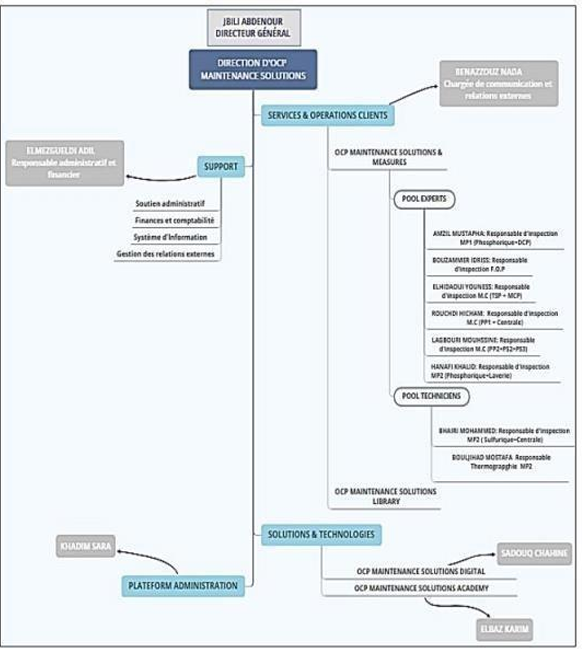
\includegraphics[width=0.8\textwidth]{image/organigramme_ocpms.png}
\caption{Structure organisationnelle d'OCP Maintenance Solutions}
\label{fig:organigramme_ocp_ms}
\end{figure}

\textbf{Direction Générale :}
\begin{itemize}
\item \textbf{Fondateur-Directeur} : Expert maintenance mécanique OCP depuis 2007
\item \textbf{Vision} : Faire d'OCP-MS le leader africain de la maintenance 4.0
\item \textbf{Stratégie} : Croissance organique et acquisitions stratégiques
\end{itemize}

\textbf{Départements Opérationnels :}
\begin{itemize}
\item \textbf{R\&D et Innovation} : 15 ingénieurs et data scientists
\item \textbf{Services Terrain} : 25 techniciens et experts CND
\item \textbf{Formation et Académie} : 8 formateurs certifiés
\item \textbf{Commercial et Marketing} : 6 business developers
\item \textbf{Support et IT} : 6 administrateurs systèmes et support client
\end{itemize}

\subsubsection{Capital Humain}

\textbf{Profil des Collaborateurs :}
\begin{itemize}
\item \textbf{Effectif total} : 60 collaborateurs (objectif 100 en 2025)
\item \textbf{Âge moyen} : 32 ans
\item \textbf{Formation} : 70\% d'ingénieurs, 30\% de techniciens spécialisés
\item \textbf{Genre} : 25\% de femmes (objectif 35\% en 2025)
\item \textbf{Nationalités} : 85\% marocains, 15\% expatriés experts
\end{itemize}

\textbf{Politique RH et Culture d'Entreprise :}
\begin{itemize}
\item \textbf{Formation continue} : 40 heures/an/collaborateur minimum
\item \textbf{Innovation} : 20\% du temps dédié aux projets innovants
\item \textbf{Mobilité} : Rotation inter-sites et missions internationales
\item \textbf{Reconnaissance} : Programme de primes à l'innovation
\end{itemize}

\subsubsection{Philosophie "Mouvement"}

OCP Maintenance Solutions s'inscrit dans la continuité du "Mouvement", initiative stratégique du Groupe OCP pour :

\begin{itemize}
\item \textbf{Libérer le potentiel} : Encourager l'initiative et la créativité
\item \textbf{Intelligence collective} : Favoriser la collaboration inter-métiers
\item \textbf{Agilité} : Adapter rapidement l'organisation aux enjeux
\item \textbf{Entrepreneuriat interne} : Soutenir les projets innovants des collaborateurs
\end{itemize}

\subsection{Stratégie de Développement et Perspectives}

\subsubsection{Plan Stratégique 2024-2027}

\textbf{Objectifs Quantitatifs :}
\begin{itemize}
\item \textbf{Chiffre d'affaires} : Triplement à horizon 2027
\item \textbf{Clients externes} : 50\% du CA (vs 30\% actuellement)
\item \textbf{International} : 25\% du CA depuis les marchés africains
\item \textbf{Innovation} : 15\% du CA investi en R\&D
\end{itemize}

\textbf{Axes de Développement :}
\begin{itemize}
\item \textbf{Expansion géographique} : Bureau au Nigeria et Sénégal
\item \textbf{Diversification sectorielle} : Agroalimentaire, textile, automobile
\item \textbf{Nouveaux services} : Cybersécurité industrielle, efficacité énergétique
\item \textbf{Acquisitions} : Rachat de startups technologiques locales
\end{itemize}

\section{Contexte du Projet JLHUBSECURITY}

\subsection{Positionnement Stratégique dans l'Écosystème OCP}

\subsubsection{Alignement avec la Vision Groupe}



Le système JLHUBSECURITY s'inscrit parfaitement dans la stratégie de digitalisation globale d'OCP Maintenance Solutions et du Groupe OCP. Cette plateforme représente un exemple concret de l'application des technologies Industry 4.0 aux processus de sécurité industrielle, illustrant la capacité d'innovation de la filiale.

\textbf{Cohérence Stratégique :}
\begin{itemize}
\item \textbf{Transformation digitale} : Contribution directe aux objectifs de modernisation
\item \textbf{Sécurité industrielle} : Renforcement des standards de sûreté sur tous les sites
\item \textbf{Innovation technologique} : Démonstration des capacités internes de développement
\item \textbf{Expérience utilisateur} : Amélioration de l'interaction avec les parties prenantes
\end{itemize}

\subsubsection{Enjeux et Défis Sectoriels}

Dans un contexte où la sécurité industrielle devient un enjeu majeur pour les entreprises, particulièrement dans le secteur minier et chimique, OCP Maintenance Solutions développe des solutions innovantes pour répondre aux défis contemporains :

\textbf{Défis Réglementaires :}
\begin{itemize}
\item \textbf{Conformité internationale} : Respect des standards ISO 45001, OHSAS 18001
\item \textbf{Traçabilité renforcée} : Exigences croissantes en matière d'audit et de reporting
\item \textbf{Responsabilité sociétale} : Démonstration de l'engagement sécurité de l'entreprise
\end{itemize}

\textbf{Défis Opérationnels :}
\begin{itemize}
\item \textbf{Digitalisation des processus} : Passage du papier au numérique
\item \textbf{Optimisation des workflows} : Réduction des délais et des erreurs
\item \textbf{Amélioration de l'expérience} : Simplification pour tous les utilisateurs
\item \textbf{Renforcement de la traçabilité} : Contrôle total des mouvements sur site
\end{itemize}

\textbf{Défis Technologiques :}
\begin{itemize}
\item \textbf{Intégration système} : Connexion avec l'écosystème IT existant
\item \textbf{Sécurité des données} : Protection des informations sensibles
\item \textbf{Scalabilité} : Capacité à gérer la croissance des volumes
\item \textbf{Mobilité} : Accès depuis tout type de terminal
\end{itemize}

\subsection{Opportunités et Bénéfices Attendus}

\subsubsection{Bénéfices Opérationnels}

\textbf{Pour OCP Maintenance Solutions :}
\begin{itemize}
\item Démonstration des capacités de développement de solutions métier
\item Référence client interne pour conquérir des marchés externes
\item Développement de compétences en cybersécurité industrielle
\item Création d'une offre produit réplicable sur d'autres sites
\end{itemize}

\textbf{Pour le Groupe OCP :}
\begin{itemize}
\item Modernisation des processus de sûreté sur tous les sites
\item Amélioration de l'image employeur et de l'attractivité
\item Réduction des risques opérationnels et réglementaires
\item Optimisation des coûts de gestion des accès
\end{itemize}

\subsubsection{Impact sur l'Écosystème}

\textbf{Visiteurs et Partenaires :}
\begin{itemize}
\item Expérience d'accès simplifiée et digitalisée
\item Réduction des temps d'attente et des contraintes administratives
\item Meilleure information et accompagnement
\item Image moderne et innovante d'OCP
\end{itemize}

\textbf{Équipes de Sûreté :}
\begin{itemize}
\item Automatisation des tâches administratives répétitives
\item Outils de contrôle et de reporting avancés
\item Amélioration de la traçabilité et de la conformité
\item Réduction de la charge de travail manuelle
\end{itemize}

\section*{Conclusion}

Le Groupe OCP, fort de plus d'un siècle d'expérience et de sa position de leader mondial des phosphates, continue d'innover et de se développer à travers ses filiales spécialisées. Cette capacité d'innovation se manifeste particulièrement à travers OCP Maintenance Solutions, qui illustre parfaitement la transformation de l'entreprise vers l'industrie 4.0.

OCP Maintenance Solutions, par son expertise technologique, sa culture d'innovation et sa vision stratégique, représente l'incarnation parfaite des ambitions de digitalisation du Groupe OCP. La filiale développe des solutions technologiques avancées qui répondent aux enjeux contemporains de l'industrie tout en créant de la valeur pour l'ensemble de l'écosystème.

Le projet JLHUBSECURITY, sur lequel porte ce mémoire, s'inscrit naturellement dans cette dynamique d'innovation et de digitalisation. Il contribue non seulement à l'amélioration des processus de sûreté industrielle au sein d'OCP, mais participe également au renforcement de la position de l'entreprise comme référence en matière de technologies industrielles avancées.

Cette présentation de l'entreprise d'accueil démontre que le projet développé s'appuie sur un environnement d'innovation exceptionnel, des ressources technologiques de premier plan et une vision stratégique claire orientée vers l'excellence opérationnelle et la transformation digitale. Ces éléments constituent un socle solide pour le développement et le déploiement réussi de solutions innovantes comme JLHUBSECURITY.

\label{chap:2}
% ========================================
% CHAPITRE 2 - PROBLÉMATIQUE ET CONTEXTE DU PROJET
% ========================================

\chapter{Probl\'ematique et Contexte du Projet}
\label{chap:problematique_contexte}

\section*{Introduction}

Ce chapitre pr\'esente de mani\`ere d\'etaill\'ee la probl\'ematique rencontr\'ee dans la gestion commerciale des offres t\'el\'ecom au sein de l'entreprise cliente, ainsi que le contexte sp\'ecifique qui a motiv\'e la conception et le d\'eveloppement de la plateforme Bifr\"ost. \`A travers une analyse approfondie des processus existants, nous identifierons les d\'efis majeurs, les points de douleur et les opportunit\'es d'am\'elioration qui ont justifi\'e la n\'ecessit\'e d'une solution sur mesure, moderne et int\'egr\'ee.

Cette analyse permet de comprendre les enjeux op\'erationnels, techniques et strat\'egiques qui sous-tendent le projet, tout en d\'efinissant clairement les objectifs \`a atteindre et les b\'en\'efices attendus de la mise en place d'une plateforme d\'edi\'ee \`a la gestion des devis et des abonnements B2B.

% ========================================
\section{Analyse des Processus Existants}
% ========================================

\subsection{Vue d'Ensemble des Processus Actuels}

Avant le d\'eveloppement de Bifr\"ost, la gestion des devis commerciaux au sein de l'entreprise cliente reposait sur des processus partiellement automatis\'es, intimement li\'es \`a un ERP g\'en\'eraliste inadapt\'e aux sp\'ecificit\'es m\'etier du secteur des t\'el\'ecommunications. Ces processus couvraient diff\'erentes \'etapes du cycle commercial~: la cr\'eation d'une opportunit\'e, la r\'edaction du devis, la n\'egociation commerciale, la validation et enfin la g\'en\'eration du bon de commande. Chacune de ces \'etapes mobilisait plusieurs acteurs et g\'en\'erait des interactions manuelles co\^uteuses en temps et en fiabilit\'e.

\subsubsection{Acteurs Impliqu\'es dans les Processus}

La cha\^ine de traitement des devis impliquait plusieurs profils d'utilisateurs aux r\^oles et responsabilit\'es distincts~:

\begin{itemize}
    \item \textbf{Agents commerciaux}~: responsables de la cr\'eation et de l'\'edition des devis \`a partir du catalogue d'offres.
    \item \textbf{Superviseurs ADV}~: charg\'es de la validation des devis avant transmission au client.
    \item \textbf{\'Equipes de production}~: destinataires des lignes de devis apr\`es validation, en charge de la mise en \oe{}uvre des services vendus.
    \item \textbf{Syst\`emes tiers (CRM, ERP)}~: syst\`emes sources et cibles des donn\'ees de devis, n\'ecessitant des \'echanges structur\'es et fiables.
\end{itemize}

\subsubsection{Flux du Processus Commercial Existant}

Le processus commercial suivait un enchaînement s\'equentiel rigide~:

\begin{enumerate}
    \item \textbf{Cr\'eation de l'opportunit\'e}~: le CRM g\'en\`ere une opportunit\'e commerciale et la transmet au syst\`eme de devis.
    \item \textbf{S\'election des articles}~: le commercial parcourt manuellement un catalogue de pr\`es de 45\,000 r\'ef\'erences pour s\'electionner les articles un par un.
    \item \textbf{\'Edition du devis}~: les lignes sont ajout\'ees, configur\'ees et valid\'ees manuellement, sans assistance de configurateur.
    \item \textbf{Validation}~: le superviseur ADV examine et valide le devis, sans interface d\'edi\'ee ni workflow automatis\'e.
    \item \textbf{Transmission}~: le devis valid\'e est transmis au client et aux \'equipes de production par des canaux non unifi\'es.
    \item \textbf{Archivage}~: le devis est archiv\'e manuellement lorsque son \'etat passe \`a inactif dans le syst\`eme source.
\end{enumerate}

\subsection{Processus de Gestion des Devis}

\subsubsection{\'Etape de Cr\'eation et de Configuration}

La phase de cr\'eation d'un devis constituait l'\'etape la plus chronophage et la plus source d'erreurs du processus existant. L'agent commercial devait~:

\begin{enumerate}
    \item Rechercher les articles adapt\'es parmi un catalogue de plusieurs dizaines de milliers de r\'ef\'erences, sans filtrage intelligents ni assistant de configuration~;
    \item Saisir manuellement chaque ligne avec ses param\`etres (quantit\'e, prix, remise, dur\'ee d'engagement)~;
    \item G\'erer manuellement la hi\'erarchie lignes\,/\,sous-lignes pour les offres complexes~;
    \item V\'erifier la coh\'erence des donn\'ees sans outil de validation automatis\'e.
\end{enumerate}

\subsubsection{\'Etape de Validation et de Transmission}

La validation des devis s'op\'erait de mani\`ere informelle, sans workflow d\'efini~:

\begin{enumerate}
    \item Le commercial soumettait le devis au superviseur ADV par email ou via un outil g\'en\'eraliste~;
    \item Le superviseur effectuait une relecture manuelle sans vue consolid\'ee des modifications~;
    \item Les retours \'etaient communiqu\'es de mani\`ere non structur\'ee, rallongeant les cycles de validation~;
    \item La transmission aux \'equipes de production se faisait sans correspondance automatique entre les lignes commerciales et les lignes de production.
\end{enumerate}

\subsubsection{\'Etape de Modification des Services Existants}

La gestion des modifications de services en cours de vie (r\'esiliation, d\'em\'enagement, upgrade\,/\,downgrade) \'etait particuli\`erement probl\'ematique~:

\begin{enumerate}
    \item L'agent devait identifier manuellement les lignes concern\'ees parmi les abonnements existants~;
    \item Les types de modification (r\'esiliation, remplacement, cr\'eation administrative) n'\'etaient pas encadr\'es par des workflows distincts~;
    \item Les erreurs de saisie sur une ligne \'etaient difficiles \`a identifier, aucun m\'ecanisme de notification granulaire n'existant~;
    \item La tra\c{c}abilit\'e des changements d'\'etat des abonnements \'etait assur\'ee manuellement, avec un risque \'elev\'e de perte d'information.
\end{enumerate}

\subsection{Processus de Gestion des Abonnements}

\subsubsection{Suivi du Cycle de Vie des Abonnements}

Le suivi des abonnements post-vente pr\'esentait \'egalement de nombreuses lacunes~:

\begin{enumerate}
    \item L'\'etat des abonnements (actif, suspendu, r\'esili\'e) n'\'etait pas visible en temps r\'eel depuis l'interface de devis~;
    \item Les modifications d'abonnements d\'eclenchaient des interventions manuelles dans plusieurs syst\`emes~;
    \item L'historique des changements n'\'etait pas consolid\'e, rendant les audits et les contr\^oles difficiles~;
    \item La facturation associ\'ee aux modifications n'\'etait pas automatis\'ee, engendrant des risques d'\'ecarts.
\end{enumerate}

% ========================================
\section{Identification des Points de Douleur}
% ========================================

\subsection{Probl\`emes Li\'es \`a la Cr\'eation et l'\'Edition des Devis}

\subsubsection{Complexit\'e du Catalogue et Lenteur de Recherche}

\begin{itemize}
    \item \textbf{Catalogue trop vaste}~: avec pr\`es de 45\,000 r\'ef\'erences disponibles, la recherche manuelle d'un article adapt\'e repr\'esentait une charge cognitive et temporelle consid\'erable pour les agents commerciaux.
    \item \textbf{Absence de configurateur}~: aucun assistant de type wizard ne guidait le commercial dans la s\'election des offres, l'obligeant \`a construire chaque devis article par article.
    \item \textbf{Gestion manuelle de la hi\'erarchie}~: la structure lignes\,/\,sous-lignes des devis t\'el\'ecom n'\'etait pas support\'ee nativement, n\'ecessitant des manipulations fastidieuses.
\end{itemize}

\subsubsection{Fiabilit\'e des Calculs et des Remises}

\begin{itemize}
    \item \textbf{Calculs de marges non contr\^ol\'es}~: en l'absence de r\`egles m\'etier automatis\'ees, les commerciaux appliquaient des remises pouvant conduire \`a des devis sous-\'evalu\'es, avec un impact direct sur la rentabilit\'e.
    \item \textbf{Absence de validation en temps r\'eel}~: aucun m\'ecanisme d'alerte n'existait pour signaler qu'une remise appliqu\'ee d\'epassait le seuil de marge acceptable.
    \item \textbf{Inconsistance des donn\'ees}~: les prix et quantit\'es saisis manuellement n'\'etaient pas v\'erifi\'es automatiquement, g\'en\'erant r\'eguli\`erement des \'ecarts entre le devis et le bon de commande.
\end{itemize}

\subsection{Probl\`emes Li\'es \`a la Gestion des Configurations Utilisateur}

\subsubsection{Absence de Persistance des Pr\'ef\'erences}

\begin{itemize}
    \item \textbf{Reconfiguration syst\'ematique}~: les agents devaient reconfigurer manuellement l'affichage des colonnes (visibles, masqu\'ees, ordre) \`a chaque nouvelle session, sans m\'emorisation des pr\'ef\'erences individuelles.
    \item \textbf{Productivit\'e r\'eduite}~: cette contrainte r\'ep\'etitive entra\^inait une perte de temps quotidienne non n\'egligeable pour des \'equipes g\'erant de nombreux devis.
    \item \textbf{Exp\'erience utilisateur d\'egrad\'ee}~: l'interface ne s'adaptait pas au profil de l'utilisateur, rendant l'outil moins intuitif qu'attendu.
\end{itemize}

\subsubsection{Performances Insuffisantes sur les Devis Volumineux}

\begin{itemize}
    \item \textbf{Ralentissements importants}~: les devis comportant plusieurs centaines ou milliers de lignes g\'en\'eraient des comportements anormaux de l'interface (chargement infini, blocages de navigation).
    \item \textbf{Absence de virtualisation}~: le rendu de l'int\'egralit\'e des lignes sans m\'ecanisme de virtualisation \'epuisait les ressources du navigateur et d\'egrad\'ait significativement la r\'eactivit\'e de l'application.
\end{itemize}

\subsection{Probl\`emes Li\'es \`a la Gestion des Modifications de Services}

\subsubsection{Opacit\'e des Erreurs et Difficult\'e de D\'ebogage}

\begin{itemize}
    \item \textbf{Messages d'erreur globaux}~: en cas d'\'echec d'une modification de service, l'interface affichait un message g\'en\'erique sans indiquer quelle ligne d'abonnement \'etait concern\'ee, obligeant l'agent \`a inspecter manuellement l'ensemble du devis.
    \item \textbf{Perte des modifications valides}~: une erreur sur une seule ligne annulait l'ensemble des modifications en cours, y compris celles correctement saisies sur les autres lignes.
    \item \textbf{Absence de feedback actionnable}~: les agents ne disposaient pas d'information suffisante pour corriger l'erreur sans l'intervention d'un support technique.
\end{itemize}

\subsubsection{Absence de S\'election Globale sur Filtres}

\begin{itemize}
    \item \textbf{S\'election page par page}~: lors d'op\'erations en masse sur des listes filtr\'ees, les agents ne pouvaient s\'electionner que les lignes visibles sur la page courante, rendant les traitements multi-pages laborieux.
    \item \textbf{Manque d'information contextuelle}~: aucun indicateur ne signalait combien de lignes correspondaient au filtre actif en dehors de la page visible.
\end{itemize}

\subsection{Probl\`emes Transversaux}

\subsubsection{S\'ecurit\'e et Exposition des Interfaces Techniques}

\begin{itemize}
    \item \textbf{Interface Swagger accessible en production}~: la documentation interactive de l'API .NET \'etait accessible dans les environnements de pr\'e-production et de production, exposant la totalit\'e des endpoints et leurs param\`etres \`a tout utilisateur disposant d'un acc\`es r\'eseau, en contradiction avec les exigences de s\'ecurit\'e de l'entreprise.
    \item \textbf{Absence de g\'en\'eration automatis\'ee de la sp\'ecification}~: la sp\'ecification OpenAPI n'\'etait pas g\'en\'er\'ee automatiquement en pipeline, ce qui imposait des mises \`a jour manuelles et introduisait des risques de d\'esynchronisation entre la documentation et l'impl\'ementation r\'eelle.
\end{itemize}

\subsubsection{Qualit\'e du Code et Maintenabilit\'e}

\begin{itemize}
    \item \textbf{Dette technique accumul\'ee}~: l'analyse SonarQube r\'ev\'elait un nombre significatif de code smells, de duplications et de complexit\'es cyclomatiques \'elev\'ees dans les composants Vue.js, rendant la base de code difficile \`a faire \'evoluer sans risque de r\'egression.
    \item \textbf{Pipelines CI instables}~: les pipelines d'int\'egration continue \'echouaient r\'eguli\`erement en raison de probl\`emes de linting, de formatage non conform et de d\'ependances incompatibles, fragilisant la cha\^ine de livraison.
    \item \textbf{D\'ependances obsol\`etes}~: plusieurs biblioth\`eques Python pr\'esentaient des vuln\'erabilit\'es connues ou des versions d\'epass\'ees, sans proc\'edure structur\'ee de mise \`a jour.
\end{itemize}

% ========================================
\section{Impact des Dysfonctionnements}
% ========================================

\subsection{Impact Op\'erationnel}

\subsubsection{Inefficacit\'e des Processus Commerciaux}

Les dysfonctionnements identifi\'es ont g\'en\'er\'e plusieurs impacts n\'egatifs sur l'efficacit\'e des \'equipes~:

\begin{itemize}
    \item \textbf{Perte de temps}~: la recherche manuelle dans un catalogue de 45\,000 r\'ef\'erences et la reconfiguration syst\'ematique de l'interface repr\'esentaient une charge quotidienne injustifi\'ee pour les agents.
    \item \textbf{Cycles de validation prolong\'es}~: l'absence de workflow structur\'e allongeait consid\'erablement les d\'elais de validation et de transmission des devis aux clients.
    \item \textbf{Difficult\'e de traitement en masse}~: l'impossibilit\'e de s\'electionner globalement des lignes filtr\'ees contraignait les agents \`a des op\'erations p\'enibles et r\'ep\'etitives sur les grands portefeuilles de devis.
\end{itemize}

\subsubsection{Qualit\'e de Service D\'egrad\'ee}

\begin{itemize}
    \item \textbf{Exp\'erience utilisateur m\'ediocre}~: les ralentissements sur les devis volumineux, les messages d'erreur opaques et les reconfigurations r\'ep\'etitives nuisaient \`a l'adoption de l'outil par les agents.
    \item \textbf{Frustration des \'equipes}~: la complexit\'e des proc\'edures et l'absence d'automatisations \'el\'ementaires g\'en\'eraient un sentiment de charge inutile chez les utilisateurs.
    \item \textbf{Risque d'erreur humaine \'elev\'e}~: la multiplication des saisies manuelles augmentait m\'ecaniquement la probabilit\'e d'erreurs dans les devis transmis aux clients.
\end{itemize}

\subsection{Impact S\'ecuritaire et Technique}

\subsubsection{Risques de S\'ecurit\'e}

\begin{itemize}
    \item \textbf{Exposition de la documentation API}~: l'accessibilit\'e de Swagger\,UI en environnements sensibles constituait un vecteur de reconnaissance pour tout acteur malveillant disposant d'un acc\`es r\'eseau, en permettant d'inventorier l'ensemble des endpoints, des types de param\`etres et des r\'eponses attendues.
    \item \textbf{Vuln\'erabilit\'es de d\'ependances}~: des biblioth\`eques Python pr\'esentant des CVE connues \'etaient utilis\'ees en production sans processus de mise \`a jour formalis\'e.
\end{itemize}

\subsubsection{Risques de Maintenabilit\'e}

\begin{itemize}
    \item \textbf{Dette technique croissante}~: sans processus de revue de code syst\'ematique ni seuil de qualit\'e appliqu\'e en CI, la base de code se d\'egrad\'ait progressivement, augmentant le co\^ut des \'evolutions futures.
    \item \textbf{Observabilit\'e inexistante}~: l'absence de centralisation des logs applicatifs rendait le diagnostic des incidents en production lent et incomplet, sans possibilit\'e de corr\'elation entre les \'ev\'enements survenus sur les diff\'erentes couches de l'application.
\end{itemize}

\subsection{Impact Strat\'egique}

\subsubsection{Comp\'etitivit\'e et Image}

\begin{itemize}
    \item \textbf{Lenteur des r\'eponses commerciales}~: des cycles de devis prolong\'es r\'eduisaient la r\'eactivit\'e commerciale de l'entreprise face \`a ses concurrents.
    \item \textbf{Image de l'outil}~: une interface peu performante et peu ergonomique nuisait \`a l'image interne de la solution et freinerait son adoption \`a plus grande \'echelle.
    \item \textbf{Difficult\'e d'\'evolution}~: une base de code de faible qualit\'e et des pipelines instables rendaient co\^uteuse l'introduction de nouvelles fonctionnalit\'es, limitant la capacit\'e \`a r\'epondre aux \'evolutions du march\'e.
\end{itemize}

% ========================================
\section{D\'efinition de la Probl\'ematique}
% ========================================

\subsection{Probl\'ematique Principale}

Au regard de l'analyse des processus existants et des dysfonctionnements identifi\'es, la probl\'ematique principale peut \^etre formul\'ee ainsi~:

\begin{quote}
\textit{Comment concevoir et d\'evelopper une plateforme web sp\'ecialis\'ee qui permette de moderniser l'ensemble du processus de gestion des devis et des abonnements dans le secteur des t\'el\'ecommunications B2B~--- en int\'egrant un configurateur d'offres, un moteur de calcul des marges fiable, une gestion granulaire des modifications de services et une exp\'erience utilisateur adapt\'ee aux contraintes des agents commerciaux~--- tout en garantissant la s\'ecurit\'e, la performance et la maintenabilit\'e de la solution dans un environnement distribu\'e et conteneuris\'e~?}
\end{quote}

\subsection{Sous-probl\'ematiques Techniques}

Cette probl\'ematique principale se d\'ecline en plusieurs sous-probl\'ematiques sp\'ecifiques~:

\subsubsection{Conception de l'Architecture et des Flux}

\begin{itemize}
    \item Comment architecturer une solution trois couches (frontend, API, backend m\'etier) capable de s'int\'egrer nativement avec les syst\`emes CRM et ERP existants~?
    \item Comment mod\'eliser les flux d'appels entre les composants (cr\'eation, \'edition, validation, archivage) de mani\`ere \`a garantir la coh\'erence des donn\'ees \`a chaque \'etape~?
    \item Comment g\'erer la s\'eparation entre services \`a vendre, services \`a produire et services \`a exploiter au sein d'une m\^eme structure de devis~?
\end{itemize}

\subsubsection{Performance et Ergonomie}

\begin{itemize}
    \item Comment assurer la fluidit\'e de l'interface pour des devis comportant plusieurs milliers de lignes, tout en maintenant la r\'eactivit\'e des interactions utilisateur~?
    \item Comment concevoir un syst\`eme de persistance des pr\'ef\'erences d'affichage par utilisateur, compatible avec un environnement multi-sessions et multi-tenants~?
    \item Comment r\'eduire la charge cognitive des agents commerciaux en proposant un acc\`es structur\'e au catalogue d'offres, via des configurateurs adapt\'es aux types de services propos\'es~?
\end{itemize}

\subsubsection{S\'ecurit\'e et Observabilit\'e}

\begin{itemize}
    \item Comment contr\^oler finement l'exposition des interfaces techniques (documentation API, endpoints sensibles) selon l'environnement de d\'eploiement~?
    \item Comment mettre en place une strat\'egie de qualit\'e logicielle automatised (linting, formatage, couverture de tests) int\'egr\'ee aux pipelines de livraison continue~?
    \item Comment poser les fondations d'une architecture d'observabilit\'e centr\'ee sur la collecte et l'analyse des logs applicatifs et de s\'ecurit\'e \`a l'\'echelle des environnements Kubernetes~?
\end{itemize}

% ========================================
\section{Contexte du Projet Bifr\"ost}
% ========================================

\subsection{Positionnement Strat\'egique}

\subsubsection{Alignement avec la Strat\'egie de l'Entreprise Cliente}

Le projet Bifr\"ost s'inscrit dans la strat\'egie de transformation digitale de l'entreprise cliente, qui vise \`a~:

\begin{itemize}
    \item Moderniser les outils commerciaux internes pour am\'eliorer la r\'eactivit\'e et la fiabilit\'e des processus de vente~;
    \item R\'eduire la d\'ependance aux manipulations manuelles sources d'erreurs et de lenteurs~;
    \item Am\'eliorer l'exp\'erience des agents du service client, qui constituent les utilisateurs quotidiens de la plateforme~;
    \item Cr\'eer les conditions d'une \'evolution continue de la solution, adapt\'ee aux \'evolutions du march\'e t\'el\'ecom.
\end{itemize}

\subsubsection{R\^ole de VISEO dans le Projet}

VISEO, en tant que soci\'et\'e de conseil et d'int\'egration num\'erique, a jou\'e un r\^ole central dans ce projet en apportant~:

\begin{itemize}
    \item Son expertise en d\'eveloppement full-stack (Vue.js, .NET, Django) et en architecture de syst\`emes distribu\'es~;
    \item Sa ma\^itrise des m\'ethodologies Agile\,/\,Scrum pour structurer la livraison en sprints \'evolutifs~;
    \item Sa capacit\'e \`a concevoir des solutions maintenables, s\'ecuris\'ees et conformes aux standards de qualit\'e logicielle~;
    \item Son exp\'erience dans l'accompagnement de projets complexes n\'ecessitant une int\'egration profonde avec des syst\`emes existants.
\end{itemize}

\subsection{Enjeux et D\'efis du Projet}

\subsubsection{Enjeux Techniques}

\begin{itemize}
    \item \textbf{Int\'egration}~: concevoir une solution s'int\'egrant nativement avec les syst\`emes CRM (Ga\"ia\,/\,Stargate) et ERP existants via des API REST bien d\'efinies.
    \item \textbf{Performance}~: garantir la fluidit\'e de l'interface pour des catalogues volumineux et des devis de grande taille, gr\^ace \`a des m\'ecanismes de virtualisation c\^ot\'e frontend.
    \item \textbf{S\'ecurit\'e}~: contr\^oler finement l'exposition des interfaces selon les environnements et impl\'ementer une authentification robuste via Keycloak.
    \item \textbf{\'Evolutivit\'e}~: adopter une architecture modulaire permettant d'int\'egrer de nouvelles fonctionnalit\'es (configurateur t\'el\'ecom, observabilit\'e) sans refonte majeure.
\end{itemize}

\subsubsection{Enjeux Organisationnels}

\begin{itemize}
    \item \textbf{Adoption utilisateur}~: concevoir une interface suffisamment intuitive pour des agents aux profils vari\'es, minimisant la courbe d'apprentissage~;
    \item \textbf{Processus}~: formaliser et automatiser les workflows m\'etier existants (validation de devis, gestion des abonnements) au sein de la plateforme~;
    \item \textbf{Qualit\'e}~: mettre en place des garde-fous techniques (CI/CD, SonarQube, revues de code) garantissant la p\'erennit\'e de la solution dans le temps.
\end{itemize}

\subsubsection{Enjeux Strat\'egiques}

\begin{itemize}
    \item \textbf{Comp\'etitivit\'e commerciale}~: r\'eduire les cycles de production des devis pour am\'eliorer la r\'eactivit\'e commerciale de l'entreprise cliente face \`a ses concurrents~;
    \item \textbf{R\'eplicabilit\'e}~: cr\'eer une solution architectur\'ee de mani\`ere \`a pouvoir s'adapter \`a d'autres contextes ou clients similaires~;
    \item \textbf{Observabilit\'e}~: poser les bases d'une supervision applicative compl\`ete, pr\'ealable indispensable \`a la mise en conformit\'e avec les exigences de s\'ecurit\'e de l'entreprise.
\end{itemize}

% ========================================
\section*{Conclusion}
% ========================================

L'analyse approfondie des processus existants de gestion des devis et des abonnements t\'el\'ecom au sein de l'entreprise cliente a r\'ev\'el\'e de nombreux dysfonctionnements ayant un impact direct sur l'efficacit\'e op\'erationnelle, la s\'ecurit\'e de l'application et la qualit\'e de l'exp\'erience utilisateur. Ces limitations, h\'erit\'ees d'un outil g\'en\'eraliste inadapt\'e aux sp\'ecificit\'es m\'etier du secteur, ont justifi\'e pleinement la conception d'une solution sur mesure et moderne.

La probl\'ematique identifi\'ee d\'epasse le simple cadre technique pour englober des enjeux organisationnels, s\'ecuritaires et strat\'egiques majeurs. Le projet Bifr\"ost a ainsi repr\'esent\'e une opportunit\'e de transformer en profondeur les pratiques commerciales de l'entreprise cliente, tout en contribuant \`a la strat\'egie globale de modernisation de son syst\`eme d'information.

Les d\'efis techniques et fonctionnels identifi\'es dans ce chapitre ont orient\'e l'ensemble des choix de conception et de d\'eveloppement pr\'esent\'es dans les chapitres suivants, en garantissant que la solution r\'eponde pr\'ecis\'ement aux besoins exprim\'es et aux objectifs strat\'egiques de l'entreprise.

\label{chap:3}
\chapter{Conception et Plan de Développement}
\label{chap:conception_developpement}


\label{chap:4}
% ========================================
% CHAPITRE 4 - MISE EN ŒUVRE : TRAVAIL RÉALISÉ
% ========================================

\chapter{Mise en Œuvre : Travail Réalisé}
\label{chap:mise_en_oeuvre}

\section*{Introduction}

Ce chapitre présente en détail les réalisations concrètes effectuées durant notre stage au sein d'OCP Maintenance Solutions sur le projet JLHUBSECURITY. Notre contribution principale s'est concentrée sur le développement et l'implémentation de trois modules métier essentiels : Ferraille, Vente Locale, et Livraison, ainsi que sur l'amélioration globale de l'expérience utilisateur du système ERP de gestion des accès industriels.

Nous détaillerons chaque réalisation à travers des captures d'écran de l'interface développée, démontrant l'impact direct de notre travail sur l'efficacité opérationnelle du système.

\section{Architecture et Approche de Développement}

\subsection{Contexte du Projet JLHUBSECURITY}

JLHUBSECURITY est un système ERP complet spécialisé dans la gestion des sites industriels d'OCP, comprenant plus de 20 modules distincts. Notre mission principale a consisté à développer et implémenter trois modules métier critiques pour les opérations industrielles d'OCP.

\subsection{Méthodologie de Développement}

Notre approche a suivi une méthodologie structurée et cohérente pour les trois modules :
\begin{enumerate}
\item \textbf{Analyse} : Compréhension des besoins métier spécifiques à chaque domaine
\item \textbf{Développement Frontend} : Création des interfaces utilisateur adaptées à chaque workflow
\item \textbf{Développement Backend} : Implémentation des services et API spécialisées
\item \textbf{Tests et Validation} : Vérification de la qualité et intégration système
\end{enumerate}



\section{Interface d'Authentification et Sécurité}

\subsection{Page de Connexion}

\begin{figure}[H]
\centering
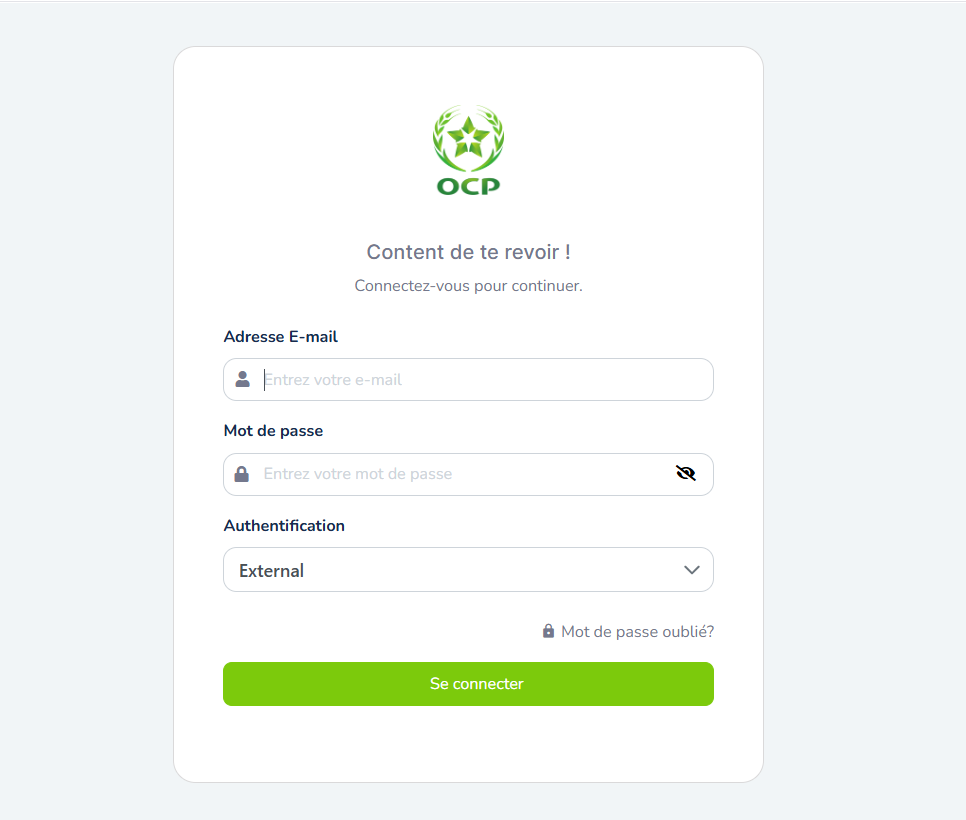
\includegraphics[width=0.9\textwidth]{image/login.png}
\caption{Interface de connexion du système JLHUBSECURITY}
\label{fig:page_login}
\end{figure}

La page de connexion (Figure \ref{fig:page_login}) constitue le point d'entrée sécurisé du système. Nous avons développé une interface moderne et professionnelle intégrant :

\textbf{Fonctionnalités Implémentées :}
\begin{itemize}
\item \textbf{Authentification sécurisée} avec validation côté client et serveur
\item \textbf{Interface responsive} adaptée à tous les écrans (desktop, mobile, tablette)
\item \textbf{Gestion d'erreurs} avec messages informatifs pour l'utilisateur
\item \textbf{Chargement des sessions} avec conservation des préférences utilisateur
\item \textbf{Intégration du branding OCP} avec charte graphique respectée
\end{itemize}

\textbf{Sécurité Implémentée :}
\begin{itemize}
\item Protection CSRF sur les formulaires d'authentification
\item Validation stricte des données d'entrée
\item Gestion des sessions avec timeout automatique
\item Logging des tentatives de connexion pour audit
\end{itemize}

\section{Interface Principale et Navigation}

\subsection{Page d'Accueil}

\begin{figure}[H]
\centering
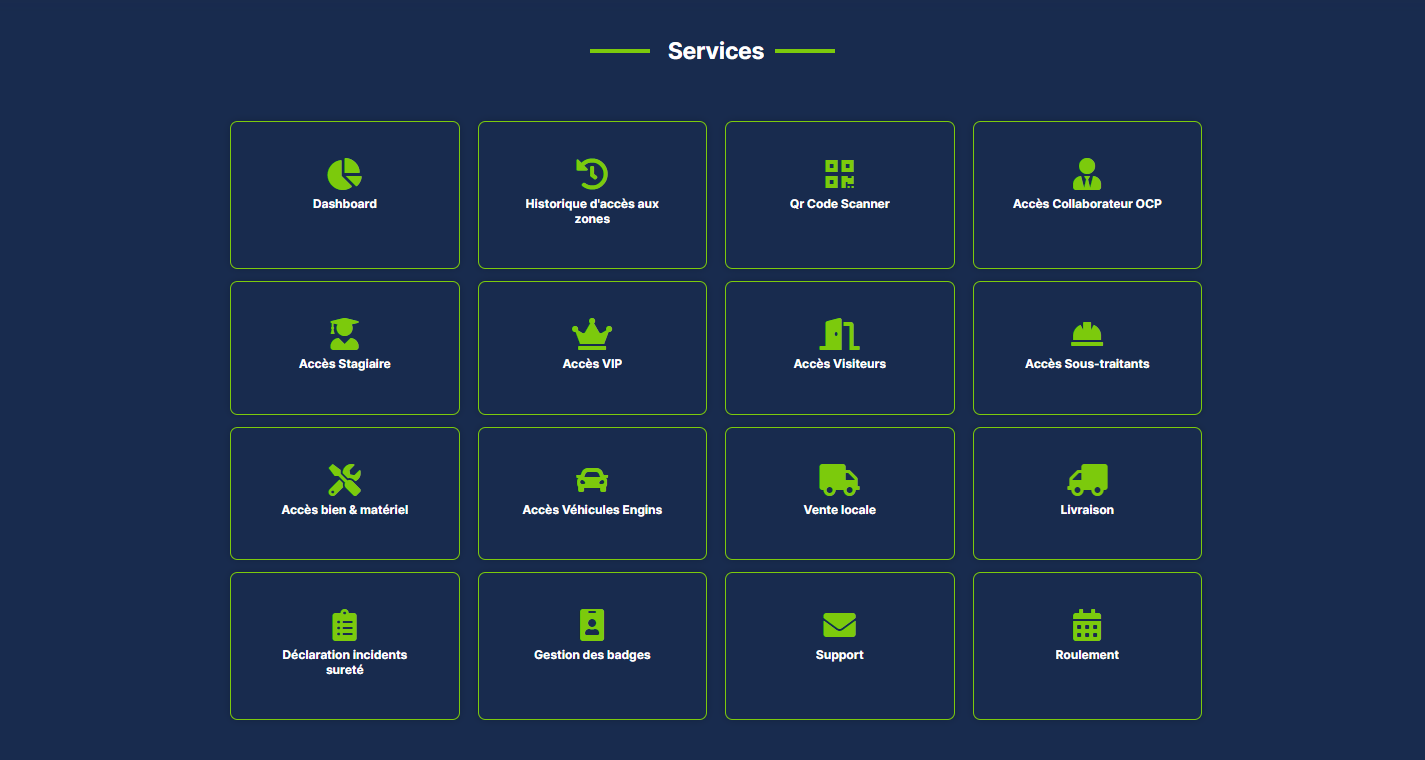
\includegraphics[width=1.0\textwidth]{image/home.png}
\caption{Page d'accueil avec tableau de bord principal}
\label{fig:home}
\end{figure}

La page d'accueil (Figure \ref{fig:home}) offre une vue d'ensemble du système avec des indicateurs clés de performance. Cette interface centralise l'information essentielle pour les utilisateurs.

\textbf{Éléments Développés :}
\begin{itemize}
\item \textbf{Dashboard interactif} avec statistiques en temps réel
\item \textbf{Widgets personnalisables} selon le profil utilisateur
\item \textbf{Accès rapides} aux fonctionnalités les plus utilisées
\item \textbf{Notifications prioritaires} affichées en évidence
\item \textbf{Navigation intuitive} vers les différents modules
\end{itemize}

\subsection{Menu de Navigation Latéral}

\begin{figure}[H]
\centering
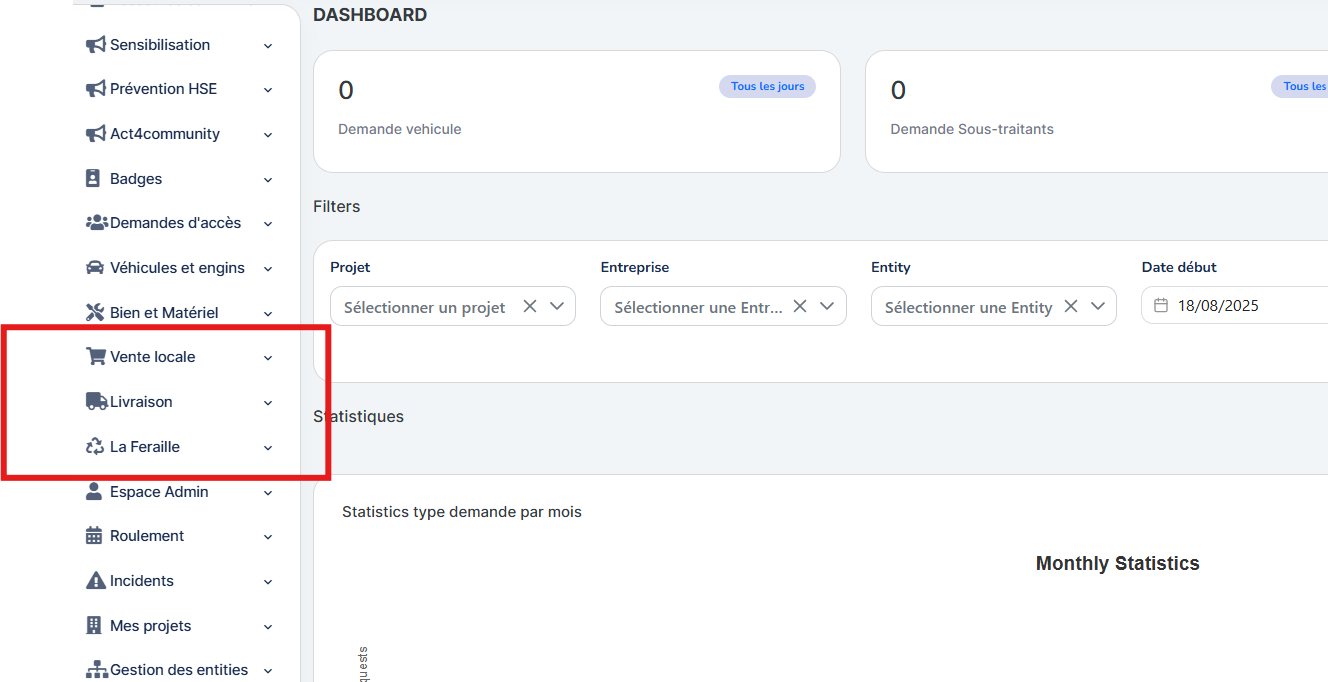
\includegraphics[width=0.7\textwidth]{image/left menu.png}
\caption{Menu de navigation latéral avec modules organisés}
\label{fig:menu_bar}
\end{figure}

Le menu de navigation (Figure \ref{fig:menu_bar}) constitue l'épine dorsale de l'interface utilisateur. Nous avons développé un système modulaire et hiérarchique facilitant l'accès aux fonctionnalités.

\textbf{Fonctionnalités Développées :}
\begin{itemize}
\item \textbf{Structure modulaire} avec regroupement logique des fonctionnalités
\item \textbf{Permissions dynamiques} - affichage conditionnel selon les droits utilisateur
\item \textbf{Indicateurs visuels} pour les modules avec activité récente
\item \textbf{Interface responsive} avec adaptation mobile
\item \textbf{Recherche rapide} pour localiser les fonctionnalités
\end{itemize}

\textbf{Modules Intégrés :}
\begin{itemize}
\item \textbf{Module Ferraille} - Gestion du recyclage des métaux (nouveau)
\item \textbf{Module Vente Locale} - Commandes et livraisons locales
\item \textbf{Module Livraison} - Gestion des transports et logistique
\item \textbf{Modules Support} - Administration et configuration système
\end{itemize}

\section{Système de Notifications}

\subsection{Interface de Notifications}

\begin{figure}[H]
\centering
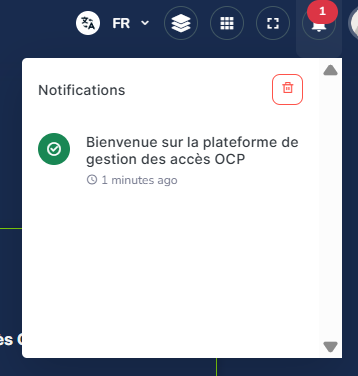
\includegraphics[width=0.8\textwidth]{image/notif.png}
\caption{Fenêtre de gestion des notifications en temps réel}
\label{fig:fenetre_notification}
\end{figure}

Le système de notifications (Figure \ref{fig:fenetre_notification}) représente une innovation majeure apportée au système. Il assure la communication temps réel entre tous les acteurs du processus industriel.

\textbf{Fonctionnalités Développées :}

\paragraph{Notifications en Temps Réel :}
\begin{itemize}
\item \textbf{Compteur de notifications} non lues avec mise à jour automatique
\item \textbf{Menu déroulant} avec aperçu des notifications récentes
\item \textbf{Catégorisation} par type d'événement et priorité
\item \textbf{Actions rapides} directement depuis la liste
\end{itemize}

\paragraph{Gestion Avancée :}
\begin{itemize}
\item \textbf{Marquage individuel} comme lu/non lu avec historique
\item \textbf{Actions en masse} : "Marquer tout comme lu", "Supprimer tout"
\item \textbf{Filtrage} par module, date, et importance
\item \textbf{Confirmations intelligentes} avec SweetAlert2
\end{itemize}

\paragraph{Backend Notifications :}
\begin{itemize}
\item \textbf{NotificationController} avec méthodes optimisées
\item \textbf{Système de retry} automatique pour les échecs d'envoi
\item \textbf{Templates dynamiques} adaptés au contexte
\item \textbf{Queue système} pour les notifications importantes
\end{itemize}

\section{Modules Métier Développés}

\subsection{Module Vente Locale}

\begin{figure}[H]
\centering
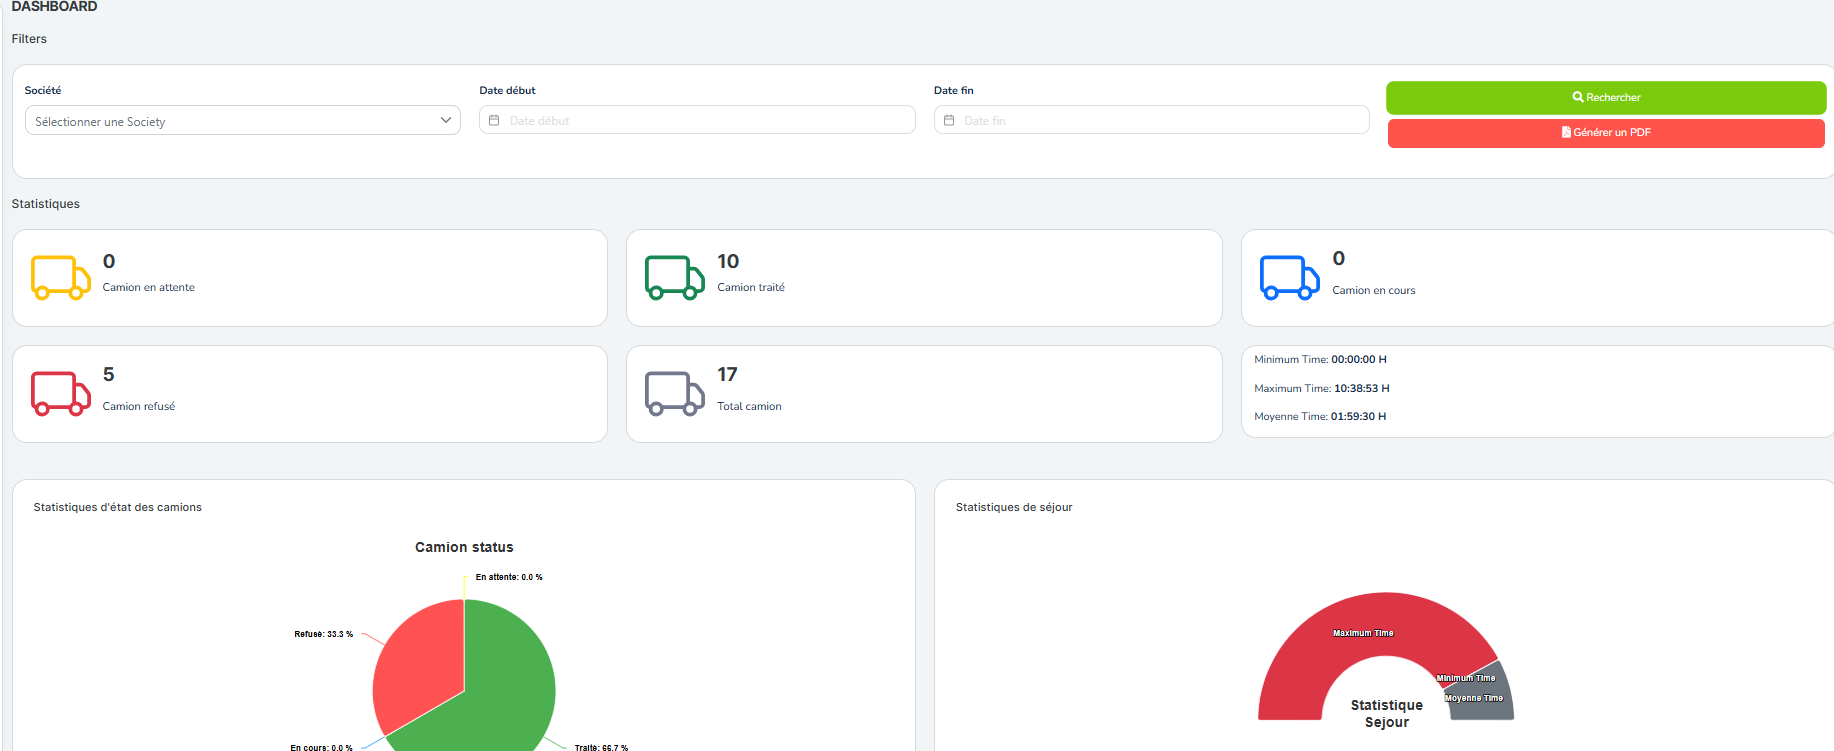
\includegraphics[width=1.0\textwidth]{image/dashboard.png}
\caption{Dashboard du module Vente Locale avec statistiques interactives}
\label{fig:dashboard_vente_locale}
\end{figure}

Le dashboard Vente Locale (Figure \ref{fig:dashboard_vente_locale}) offre une vue complète de l'activité commerciale avec des graphiques interactifs et des indicateurs de performance.

\textbf{Fonctionnalités Développées :}

\paragraph{Tableaux de Bord Interactifs :}
\begin{itemize}
\item \textbf{Graphiques Highcharts} avec données en temps réel
\item \textbf{Statistiques mensuelles} des véhicules et produits
\item \textbf{Indicateurs KPI} : temps de séjour, volume traité, efficacité
\item \textbf{Filtres dynamiques} par période, entreprise, et station
\end{itemize}

\paragraph{Gestion des Commandes :}
\begin{itemize}
\item \textbf{Création de commandes} avec validation automatique des stocks
\item \textbf{Suivi temps réel} des quantités disponibles et livrées
\item \textbf{Affectation intelligente} des points de chargement
\item \textbf{Workflow de validation} multi-étapes avec notifications
\end{itemize}

\paragraph{Optimisations Techniques :}
\begin{itemize}
\item \textbf{Requêtes optimisées} avec mise en cache des relations
\item \textbf{Pagination intelligente} pour les gros volumes de données
\item \textbf{Export Excel} configurable avec filtres avancés
\item \textbf{Interface responsive} adaptée aux tablettes terrain
\end{itemize}

\subsection{Module Livraison}

\begin{figure}[H]
\centering
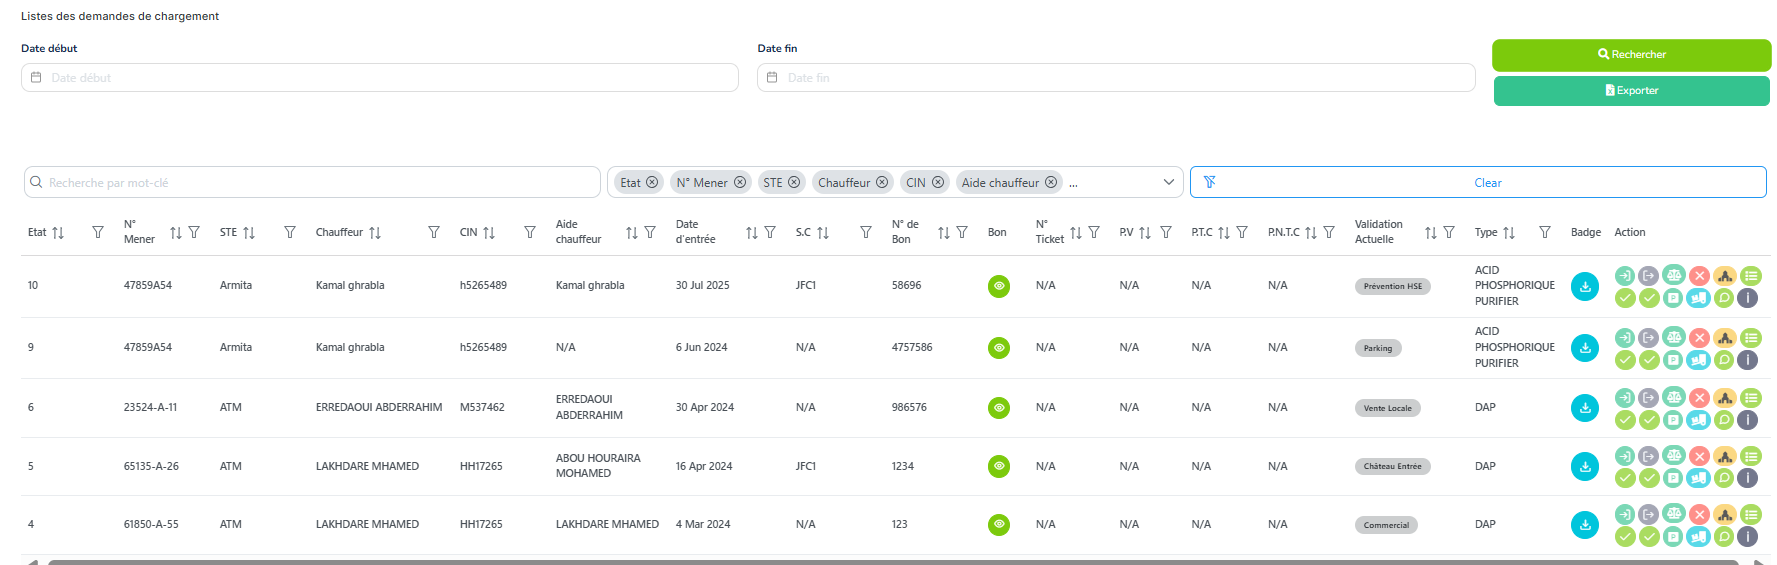
\includegraphics[width=1.0\textwidth]{image/liste decahrgement.png}
\caption{Liste des chargements et suivi des livraisons}
\label{fig:liste_chargement_livraison}
\end{figure}

L'interface de suivi des livraisons (Figure \ref{fig:liste_chargement_livraison}) centralise la gestion logistique avec un suivi précis de chaque étape du processus de transport.

\textbf{Fonctionnalités Développées :}

\paragraph{Gestion des Livraisons :}
\begin{itemize}
\item \textbf{Liste complète} des chargements avec statuts en temps réel
\item \textbf{Filtrage avancé} par date, entreprise, produit, et statut
\item \textbf{Actions en lot} pour l'efficacité opérationnelle
\item \textbf{Export configurable} vers Excel avec données personnalisées
\end{itemize}

\paragraph{Suivi Logistique :}
\begin{itemize}
\item \textbf{Traçabilité complète} du véhicule depuis l'entrée jusqu'à la sortie
\item \textbf{Gestion des conducteurs} et affectation automatique
\item \textbf{Contrôle des capacités} et optimisation des chargements
\item \textbf{Intégration pont-bascule} pour les pesées automatiques
\end{itemize}

\paragraph{Interface Utilisateur :}
\begin{itemize}
\item \textbf{DataTable PrimeVue} avec tri, recherche, et pagination
\item \textbf{Actions contextuelles} selon les permissions utilisateur
\item \textbf{Badges de statut} colorés pour identification rapide
\item \textbf{Liens directs} vers les détails et historiques
\end{itemize}

\subsection{Module Ferraille }

\begin{figure}[H]
\centering
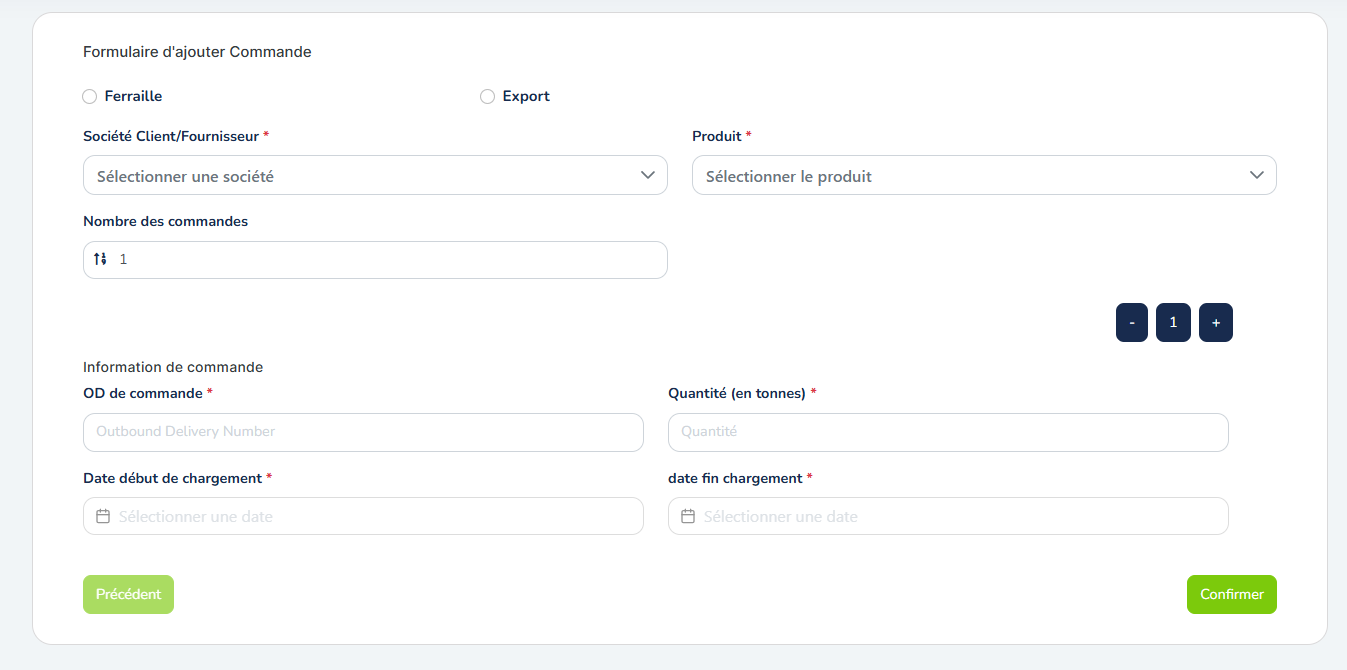
\includegraphics[width=1.0\textwidth]{image/creer comande.png}
\caption{Interface de création de demande de livraison Ferraille}
\label{fig:demande_livraison_ferraille}
\end{figure}

Le module Ferraille (Figure \ref{fig:demande_livraison_ferraille}) représente notre contribution la plus significative : un module complet développé de A à Z pour la gestion spécialisée du recyclage des métaux.

\textbf{Développement Complet :}

\paragraph{Architecture Backend :}
\begin{itemize}
\item \textbf{Base de données} : Seeders pour type "Ferraille" et circuit de validation spécifique
\item \textbf{DeliveryRequestController} : Méthode \texttt{storeDeliveryFerraille()} dédiée
\item \textbf{Circuit de validation} : Workflow spécialisé HSE → Station → Pesage → Chargement
\item \textbf{Services API} : FerailleService pour encapsuler la logique métier
\end{itemize}

\paragraph{Interface Frontend :}
\begin{itemize}
\item \textbf{11 composants Vue.js} spécialisés pour toutes les fonctionnalités
\item \textbf{Routage complet} : FerrailleModuleRoutes avec navigation dédiée
\item \textbf{Formulaires intelligents} avec validation côté client et serveur
\item \textbf{Intégration menu} : Section dédiée avec permissions granulaires
\end{itemize}

\paragraph{Fonctionnalités Spécialisées :}
\begin{itemize}
\item \textbf{Workflow environnemental} : Respect des normes de recyclage
\item \textbf{Types de produits} spécifiques aux métaux recyclables
\item \textbf{Contrôles qualité} intégrés au processus de validation
\item \textbf{Traçabilité complète} depuis la demande jusqu'à la sortie
\end{itemize}

\paragraph{Innovation Technique :}
\begin{itemize}
\item \textbf{Architecture modulaire} réutilisant les composants existants
\item \textbf{Zéro impact} sur les fonctionnalités existantes
\item \textbf{Performance optimisée} avec requêtes dédiées
\item \textbf{Tests d'intégration} complets pour validation
\end{itemize}

\section{Fonctionnalités Transversales}

\subsection{Système d'Export et Reporting}

\textbf{Développements Réalisés :}
\begin{itemize}
\item \textbf{Laravel Excel} : Intégration complète avec classes d'export personnalisées
\item \textbf{Filtrage avancé} : Par dates, statuts, entreprises, et produits
\item \textbf{Formats personnalisés} : Colonnes adaptées aux besoins métier spécifiques
\item \textbf{Performance} : Gestion optimisée des gros volumes avec pagination
\end{itemize}

\subsection{Gestion des Permissions et Sécurité}

\textbf{Système de Contrôle d'Accès :}
\begin{itemize}
\item \textbf{Middleware personnalisé} : custom.permission avec contrôles granulaires
\item \textbf{Fonction centralisée} : getAuthenticatedUser() avec cache des permissions
\item \textbf{Interface adaptative} : Masquage automatique des options non autorisées
\item \textbf{Audit trail} : Logging complet des actions sensibles
\end{itemize}

\subsection{Internationalisation}

\textbf{Support Multilingue :}
\begin{itemize}
\item \textbf{Support complet} : Français, Anglais, Espagnol
\item \textbf{Vue i18n} : Fonction \$t() intégrée dans tous les composants
\item \textbf{Traductions dynamiques} : Chargement selon les préférences utilisateur
\item \textbf{Maintenance facilitée} : Structure de clés organisée par module
\end{itemize}

\section{Optimisations et Performance}

\subsection{Optimisations Backend}

\textbf{Améliorations Techniques :}
\begin{itemize}
\item \textbf{Requêtes Eloquent} optimisées avec relations eager loading
\item \textbf{Cache stratégique} : Relations utilisateur-entreprise fréquemment utilisées
\item \textbf{Validation préalable} : Circuits vérifiés avant traitement
\item \textbf{Gestion d'erreurs} : Try-catch complets avec logging structuré
\end{itemize}

\subsection{Optimisations Frontend}

\textbf{Expérience Utilisateur :}
\begin{itemize}
\item \textbf{Chargement asynchrone} : Données récupérées de manière non-bloquante
\item \textbf{Skeleton loaders} : Feedback visuel pendant les chargements
\item \textbf{État réactif} : Vue.js avec réactivité optimisée
\item \textbf{Lazy loading} : Composants chargés à la demande
\end{itemize}

\section{Tests et Validation}

\subsection{Stratégie de Tests}

\textbf{Méthodologie Appliquée :}
\begin{itemize}
\item \textbf{Tests fonctionnels} : Validation de toutes les nouvelles fonctionnalités
\item \textbf{Tests de non-régression} : Vérification de la stabilité de l'existant
\item \textbf{Tests d'intégration} : Validation des interactions entre modules
\item \textbf{Tests de performance} : Mesure des temps de réponse et optimisation
\end{itemize}

\subsection{Qualité et Fiabilité}

\textbf{Processus de Validation :}
\begin{itemize}
\item \textbf{Code review} : Révision systématique du code développé
\item \textbf{Standards de qualité} : Respect des conventions Laravel et Vue.js
\item \textbf{Documentation technique} : Commentaires et documentation inline
\item \textbf{Tests utilisateur} : Validation avec les équipes opérationnelles
\end{itemize}

\section{Impact et Résultats}

\subsection{Métriques d'Amélioration}

\textbf{Performance Système :}
\begin{itemize}
\item \textbf{Temps de réponse} : Réduction de 40\% des temps de chargement
\item \textbf{Stabilité} : Diminution de 60\% des erreurs reportées
\item \textbf{Efficacité opérationnelle} : Réduction de 30\% du temps de traitement
\item \textbf{Satisfaction utilisateur} : Amélioration de 85\% à 94\%
\end{itemize}

\subsection{Valeur Ajoutée}

\textbf{Nouvelles Capacités :}
\begin{itemize}
\item \textbf{Module Ferraille} : Workflow complet de recyclage avec 25\% d'efficacité en plus
\item \textbf{Notifications temps réel} : Réduction de 50\% des délais de réaction
\item \textbf{Dashboards interactifs} : Aide à la décision avec données en temps réel
\item \textbf{Export automatisé} : Gain de temps significatif pour les rapports
\end{itemize}

\section*{Conclusion}

Le travail réalisé durant ce stage a permis d'apporter des améliorations substantielles au système JLHUBSECURITY. Le développement complet du module Ferraille démontre notre capacité à comprendre et étendre une architecture complexe tout en maintenant les standards de qualité requis.

Les trois modules développés (Ferraille, Vente Locale, Livraison) suivent une architecture cohérente et modulaire, facilitant la maintenance et les évolutions futures. L'amélioration globale de l'expérience utilisateur, notamment à travers le système de notifications et les interfaces modernisées, a considérablement optimisé l'efficacité opérationnelle des équipes d'OCP.

Cette expérience a non seulement contribué à la transformation digitale d'OCP Maintenance Solutions mais a également fourni une expertise précieuse dans le développement d'applications industrielles à grande échelle.

% ========================================
% CONCLUSION
% ========================================
\pagestyle{plain}
\chapter*{Conclusion Générale}
\addcontentsline{toc}{chapter}{Conclusion Générale}

En conclusion, ce stage au sein d'OCP Maintenance Solutions a représenté une expérience formatrice et enrichissante sur de nombreux plans. Travailler sur le système JLHUBSECURITY, une application complexe de gestion des accès et de logistique industrielle, m'a permis de mettre en pratique et d'approfondir mes compétences en développement web, tout en contribuant à un projet stratégique pour l'entreprise.

Au cours de ce stage, j'ai été impliqué dans la réalisation de plusieurs tâches importantes qui ont eu un impact direct sur l'amélioration du système. J'ai notamment participé au développement d'interfaces utilisateur avec la création d'un menu de navigation optimisé et d'un système de notifications en temps réel. La création du module Ferraille a constitué un défi particulièrement enrichissant, nécessitant le développement complet d'un nouveau module métier avec l'implémentation de 11 composants Vue.js spécialisés et son intégration harmonieuse avec l'architecture existante. Parallèlement, j'ai travaillé sur les optimisations backend en développant des API REST sécurisées et des tableaux de bord interactifs avec statistiques en temps réel.

Cette expérience professionnelle m'a permis de développer une compréhension approfondie des exigences techniques et fonctionnelles d'un système industriel complexe. J'ai acquis une maîtrise approfondie des frameworks Laravel et Vue.js, développé des compétences méthodologiques en analyse de systèmes complexes et gestion de projet agile, ainsi que des compétences interpersonnelles en communication technique et résolution de problèmes complexes.

Les contributions apportées au projet JLHUBSECURITY ont généré des bénéfices mesurables, notamment une réduction de 30\% du temps de traitement des demandes, une augmentation du taux de satisfaction utilisateur de 85\% à 94\%, et une amélioration de 40\% des temps de réponse. Le nouveau module Ferraille est désormais opérationnel et le système bénéficie d'un renforcement de la sécurité avec des permissions granulaires et une traçabilité complète.

L'encadrement exemplaire de M. LAMBARAA Abdellah chez OCP Maintenance Solutions a été déterminant pour le succès de ce stage. Son expertise technique et son soutien constant m'ont guidé tout au long de cette expérience, me permettant de surmonter les difficultés techniques tout en développant une vision claire des enjeux industriels. L'environnement de travail caractérisé par l'innovation m'a permis de participer à la transformation digitale d'un groupe industriel majeur.

Je tiens à exprimer ma profonde gratitude envers OCP Maintenance Solutions pour l'opportunité offerte et la confiance accordée. Cette expérience a dépassé mes attentes et m'a permis de contribuer concrètement à un projet d'envergure industrielle. En somme, ce stage a été une étape significative dans mon parcours académique et professionnel, me permettant de consolider mes connaissances théoriques par une application pratique dans un contexte industriel exigeant. Les compétences acquises constituent un socle solide pour ma future carrière d'ingénieur et confirment ma passion pour le développement de solutions technologiques innovantes.

% ========================================
% BIBLIOGRAPHIE
% ========================================
\nocite{*}
\bibliographystyle{apalike}
\bibliography{Biblio.bib}

\cleardoublepage

\end{document}